\documentclass[a4paper, 12pt]{report}
\usepackage[utf8]{inputenc}
\usepackage[T1]{fontenc}

\usepackage{xcolor}
\usepackage{afterpage}

\usepackage{relsize}
\usepackage{moresize}

\usepackage{graphicx}
\usepackage{geometry}

% [CHANGE] The title of your thesis. If your thesis has a subtitle, then this
% should appear right below the main title, in a smaller font.
\newcommand{\theTitle}{Anisotropic Quadratic Forms for \\
\vspace{0.5em}
Pooling in Deep Learning}
\newcommand{\theSubTitle}{}


% [CHANGE] Your full name. In case of multiple names, you can include their
% initials as well, e.g. "Robin G.J. van Achteren".
\newcommand{\theAuthor}{Peter Adema}

% [CHANGE] Your student ID, as this has been assigned to you by the UvA
% administration.
\newcommand{\theStudentID}{14460165}

% [CHANGE] The name of your supervisor(s). Include the titles of your supervisor(s),
% as well as the initials for *all* of his/her first names.
\newcommand{\theSupervisor}{Dr.\ ir.\ R.\ van den Boomgaard} % Dr. Ing. L. Dorst

% [CHANGE] The address of the institute at which your supervisor is working.
% Be sure to include (1) institute (is appropriate), (2) faculty (if
% appropriate), (3) organisation name, (4) organisation address (2 lines).
\newcommand{\theInstitute}{
Informatics Institute \\ %Institute for Logic, Language and Computation
Faculty of Science\\
University of Amsterdam\\
Science Park 900 \\ 
1098 XH Amsterdam 
}

% [CHANGE] The semester in which you started your thesis.
\newcommand{\theDate}{Semester 2, 2024-2025}



\usepackage[shortlabels]{enumitem}
\usepackage{graphicx}

\usepackage{hyperref}
\usepackage{amsmath}
\usepackage{amssymb}
\usepackage{amsthm}
\usepackage{mathabx}
%\usepackage{apacite}
\usepackage{caption}
\usepackage{listings}
\usepackage{xcolor}
\usepackage{array}
\usepackage{booktabs}
\def\comment#1{\color{red}#1\color{black}}
\def\gray#1{\color{gray}#1\color{black}}
\usepackage{bbold}
\DeclareMathOperator{\boxclose}{\vcenter{\hbox{$\blacksquare$}}}
\DeclareMathOperator{\boxopen}{\Box}
\definecolor{opening_red}{RGB}{169,15,70}
\definecolor{opening_blue}{RGB}{94, 79, 162}
\begin{document}
\pagestyle{empty}
\begin{center}

\vspace{2.5cm}


\begin{Huge}
% see definition at beginning of document
\theTitle
\end{Huge} \\

\vspace{0.5 cm}

\begin{Large}
\theSubTitle
\end{Large}

\vspace{1.5cm}

% see definition at beginning of document
\theAuthor\\
% see definition at beginning of document
\theStudentID

\vspace{1.5cm}

% [DO NOT CHANGE]
Bachelor thesis\\
Credits: 18 EC

\vspace{0.5cm}

% [DO NOT CHANGE] The name of the educational programme.
Bachelor \textit{Kunstmatige Intelligentie} \\
\vspace{0.25cm}

\includegraphics[width=0.075\paperwidth]{figures/uva_logo} \\
\vspace{0.1cm}

% [DO NOT CHANGE] The address of the educational programme.
University of Amsterdam\\
Faculty of Science\\
Science Park 900\\
1098 XH Amsterdam

\vspace{2cm}

\emph{Supervisor}\\

% see definition at beginning of document
\theSupervisor

\vspace{0.25cm}

% see definition at beginning of document
\theInstitute

\vspace{1.0cm}

% see definition at beginning of document
\theDate

\end{center}
\newpage



\pagenumbering{arabic}
\setcounter{page}{1}
\pagestyle{plain} 


\section*{Abstract}
Convolutional neural networks typically contain nonparametric max-pooling layers. However, using a mathematical generalisation of a max-pooling called a dilation, these max-pooling layers can be replaced with a parametrisable alternative. Previous research has shown that combining such a dilation with a (convolutional) kernel generated by an isotropic quadratic function can lead to models which perform better on simple image classification tasks. 

We extend these results using anisotropic quadratic functions, enabling kernels shaped like ellipses instead of only circles. Backed by a separate Extension report that provides an efficient implementation, we perform a series of small-scale experiments to examine the effects of anisotropy on classifier performance. We find that, for datasets analysed in preceding works, anisotropy generally improves isotropic kernels. However, an additional dataset added for this report (Fashion-MNIST) showed both dilation variants performing poorly, whereas previous research only showed positive results. 

We conclude that dilation-based poolings can improve classifier performance and that adding anisotropic kernels can further this improvement, but these outcomes are not guaranteed for all tasks and models. Further research is necessary to determine under which circumstances dilation-based poolings should be applied.

All code is available in a \href{https://github.com/p-adema/quadratic-conv}{\color{cyan}GitHub repository}.

\vfill
\section*{Acknowledgements}
I would like to thank my supervisor \theSupervisor\ for their invaluable feedback, enthusiastic guidance and cordial attitude: their comments helped guide the structure and content of this report. I also greatly appreciate the work my friends and family have done proofreading this report and their understanding during this somewhat hectic period. Without the support of those around me, this report would not have been possible to write.

\newgeometry{a4paper, textwidth=400.0pt, textheight=740.0pt}
\tableofcontents


\chapter{Introduction}
In the field of computer vision, machine learning has been successfully applied for societal benefit in various ways, ranging from analysing medical imaging data \cite{esteva2021deep, jain2015computer} to classifying agricultural produce \cite{wan2020faster, sivaranjani2022overview} and recognising license plate numbers \cite{xie2018new}. One of the primary tools used in these applications is the Convolutional Neural Network (CNN) \cite{le1990handwritten}, a type of neural network that leverages existing theoretical knowledge of image processing to learn representations of images more efficiently.

Two components are often seen within a typical CNN: the eponymous convolutional layer, which analyses the image, and a pooling layer, which compresses the image representation (see \cite{introconvnets} for an introduction). The latter pooling layer is often implemented as a max-pooling layer, which selects the highest value in a small area surrounding every point in the image. Slightly more generally, a max-pooling layer can be seen as an operation that weights neighbouring pixels around a point in the image and selects the pixel with the highest weight, but with all neighbours being weighted equally. However, this general perspective suggests the possibility of a variation on a max-pooling layer where pixels are not weighted equally: instead, pixels further away from the centre could be considered less in the selection for the maximum.

This idea has been formalised in mathematical morphology as dilation \cite{heijmans1996morphological} and in tropical geometry as a max-plus convolution \cite{maragos}. Using this formalism, a separate function $G$ (the structuring element or kernel) defines the weighting for neighbouring pixels. This function can be parameterised in various ways, but a concave function centred around the origin is typically used for G. One such function is the quadratic function $f(x)=x^T\Sigma^{-1}x$, and another is its isotropic form $f(x)=x^T(sI)^{-1}x$, with parameters $\Sigma$ and $s$ respectively \cite{Boomgaard1999NumericalSS}.

Previous studies \cite{groenendijk2022morphpool} and theses \cite{thierrybsc, koenbsc} have investigated the possibility of using such a dilation (generalised max-pooling) with an isotropic quadratic kernel as a layer within a CNN, with the parameter $s$ being learned via gradient descent (a standard optimisation method within machine learning). This previous research showed that using an isotropic quadratic kernel resulted in higher performance on a selection of small datasets. This thesis aims to expand upon this by examining the possibility of using an anisotropic quadratic kernel within the dilation, specifically whether the anisotropic parameters $\Sigma$ could also be learned via gradient descent. The expectation is that, since anisotropic quadratic kernels are again strictly more expressive than the isotropic versions, such a dilation layer would further improve performance. This report will cover the theoretical and experimental portions of this research, while implementation details are instead documented in the auxilliary Extension report: \cite{extension}.

\newpage
\section{Related work}
Modern Convolutional Neural Networks (CNNs) often use linear convolutional layers to process images and max-pooling layers to condense information and shrink the feature space \cite{introconvnets}. However, both of these operations are equivalent to a semifield convolution: the first in the linear field (with a learned kernel) and the second in the tropical-max field (with a step-function-like kernel) \cite{bellaardaxiomatic}. In \cite{bellaardaxiomatic}, Bellaard et al.\ provide an axiomatic foundation for using various semifields within the context of PDE- (continuous) CNNs but do not discuss using semifields for conventional (discrete) CNNs. 

However, the ideas underlying tropical fields are older than \cite{bellaardaxiomatic}. The field of mathematical morphology researches the shapes and forms of objects and functions, and two of the core operators within mathematical morphology are dilation (equivalent to a tropical-max / max-plus convolution) and erosion (close to a tropical-min correlation) \cite{maragos}. Heijmans provides an excellent treatment of many of the theoretical fundamentals and generalised cases of mathematical morphology in \cite{heijmans1996morphological}, with Chapter 11 describing morphology for grey-scale images, which is most similar to the convolutional operations relevant to this report. Furthermore, morphological operations with specifically a quadratic kernel are well-studied, e.g.\ Boomgaard showing in \cite{Boomgaard1999NumericalSS} that many parts of the calculation can be done in closed form without first approximating the quadratic as a fixed-size kernel.

Another paper of note regarding the efficient calculation of a convolution with an anisotropic kernel in tropical semifields may be \cite{fastanifilter}, in which Geusebroek and van de Weijer discuss how to approximate separability to perform an efficient calculation for a linear convolution with a Gaussian kernel. However, due to time constraints, this method was not implemented for the anisotropic semifield convolutions in this report.

Aside from relevant theory, there is also some more recent experimental research adjacent to this topic. Notably, \cite{qlin1, qlin2} show that a CNN that learns quadratic scale parameters for the kernels of its linear convolution can sometimes learn to perform tasks similar to those of a CNN that directly learns all kernel parameters. This adjustment significantly reduces the number of  parameters required for the linear convolutions replaced in such a way. Also close to the topic, \cite{fan2021alternative} investigate (with unfortunately unclear results) the possibility of replacing linear convolutional layers with max-plus convolutions, arguing that replacing multiplication with addition may result in models using less power.

Finally, \cite{groenendijk2022morphpool} and previous projects under Dr Boomgaard have partly investigated discrete semifield convolutions. The isotropic case --- where scales are equal in all directions --- for tropical-max fields has been relatively well-researched by \cite{thierrybsc, koenbsc}, showing minor performance increases in basic image classification tasks. However, a more general treatment of anisotropic kernels in tropical max semifields (and other semifields) is not yet present within the public domain or the UvA collection of theses.

\chapter{Background}
First, mathematical formalisms must be covered to understand the concepts discussed in later sections. These include the convolutional operator, its generalisation using semifields, and relevant semifields from mathematical morphology. Afterwards, we will discuss variations present in the convolution operator as used in Convolutional Neural Networks.

\section{Convolutional operator}
At the core of a convolutional neural network is the convolutional operation $f*g$. The general form of a continuous convolution of functions $f$ and $g$ can be written as:
\begin{align}
(f*g)(x) &= \int_{y\in\mathcal{D}} f(x-y)\; g(y)	,
\end{align}
where $\mathcal{D}$ is the (continuous) domain of $f$ and $g$. However, save for a handful of functions whose convolutions can be calculated algebraically, we are typically required to approximate this convolution in the discrete domain. In this case, we approximate the functions $f$ and $g$ by sampling them at fixed intervals, the result of which can be represented as discrete arrays $F$ and $G$. A discrete convolution could then be written as \cite{szeliski2022computer}:
\begin{align}
(F*G)[x] &= \sum_{y\in\mathcal{Y}} F[x-y]\; G[y],
\end{align}
where $\mathcal{Y}$ is the set of all indices in the domain of $F$ and $G$ (e.g.\ $\mathcal{Y}=\mathbb{Z}^2$ for infinitely large 2D images and kernels), and $G$ is typically referred to as the (convolutional) kernel.


\section{Fields and semifield convolutions}
In the convolutional operator, a part of the image is repeatedly multiplied element-wise with a kernel, and the resulting values are summed to obtain an activation for each point. However, while we typically use scalar addition and multiplication in this calculation, it is also possible to use different operators in the reduction by defining a different field in which the reduction is done. In this section, we will briefly look at the concept of fields insofar as they are relevant to implementing an alternative version of the convolutional operator.

In mathematics, a field is a set of values with a pair of operators: one operator corresponds to the concept of addition, and one operator corresponds to the concept of multiplication. Fields are, in effect, a generalisation of standard addition and multiplication on integers or reals that allow for describing a set of values other than typical scalars or an alternate method for combining typical numbers. Formally, a field can be described as a tuple $(\mathcal{F}, \oplus, \otimes)$, where the operators $\oplus$ and $\otimes$ (which we select to take the role of 'normal' + and $\times$) are of the type $\mathcal{F}\times\mathcal{F}\rightarrow\mathcal{F}$. Furthermore, the semifield operators $\oplus$ and $\otimes$ are both beholden to the field axioms: informally, a set of rules to ensure they act 'similarly' to scalar ('normal') addition and multiplication. 

These field axioms can be written as (adapted from \cite{beachy2006abstract} and \cite{bellaardaxiomatic}):
\begin{align}
\textrm{$\oplus$ is associative: }&\forall a,b,c\in \mathcal{F} &  a \oplus (b \oplus c) = (a\oplus b) \oplus c \\ 
\textrm{$\otimes$ is associative: }&\forall a,b,c\in \mathcal{F} &  a \otimes (b \otimes c) = (a\otimes b) \otimes c \\ 
\textrm{$\oplus$ is commutative: }&\forall a,b\in \mathcal{F} & a\oplus b = b  \oplus a \\
\textrm{$\otimes$ is commutative: }&\forall a,b\in \mathcal{F} & a\otimes b = b  \otimes a \\
\oplus\textrm{ has an identity: }& \exists \mathbb{0} ~\forall a\in \mathcal{F} & a\oplus \mathbb{0} = a \\ 
\otimes\textrm{ has an identity: }& \exists \mathbb{1} ~\forall a\in \mathcal{F} & a\otimes \mathbb{1} = a \\ 
\oplus\textrm{ has inverse elements: }& \forall a~\exists b\in \mathcal{F} & a\oplus b = \mathbb{0} \label{eq:additive-inverse}  \\ 
\otimes\textrm{ has inverse elements: }& \forall a~\exists b\in \mathcal{F} & a\otimes b = \mathbb{1}  \\ 
\mathbb{0} \textrm{ is absorbing for $\otimes$: }&\forall a\in \mathcal{F} & a\otimes \mathbb{0} = \mathbb{0}\\
\otimes \textrm{ distributes over $\oplus$: }&\forall a,b,c\in \mathcal{F} & a\otimes (b \oplus c) = (a\otimes b)\oplus(a\otimes c)
\end{align}
\noindent
One use case for fields in machine learning is to describe a weighted reduction --- as used in a kernel-based convolution --- more generally. To better understand this, let us return to the example of the convolutional operator. In this case, we must reduce the neighbourhood around a pixel $x$ in the image $F$, weighted by the values in the kernel $G$. While this would typically be written as:
\begin{align}
	(F*G)[x] &= \sum_{y\in\mathcal{Y}} F[x-y]\; G[y],
\intertext{
we could instead use a field $S=(\mathcal{F}, \oplus, \otimes)$ and write a similar operation:
}
	(F ~\textcircled{$*$}_S\; G)[x] &=\bigoplus_{y\in \mathcal{Y}} F[x-y] \otimes G[y] \label{eq:semifield-conv}
\end{align}
\noindent
Performing this operation does not, strictly speaking, require any of the above field axioms to hold for $\oplus$ or $\otimes$: the only relevant restriction would be that of the types being $\mathcal{F}\times\mathcal{F}\rightarrow\mathcal{F}$. However, implementing this operation for a CNN would require both operators to be differentiable and for $\mathbb{0}$ to exist (to deal with the border effects in a convolution). Furthermore, it is generally also useful for the reduction operator $\oplus$ to be both associative and commutative, as this makes the order of elements in the input irrelevant, promoting the stability of the result and allowing efficient parallel implementation of the reduction \cite{ppad}. In general, most operators we would seek to use for $\oplus$ and $\otimes$ already adhere to all semifield axioms, save for Eq. \ref{eq:additive-inverse}. As such, we will drop only Eq. \ref{eq:additive-inverse} and use semifields for generalising convolutions \cite{bellaardaxiomatic}:
\textbf{A semifield is a field, except an additive ($\oplus$) inverse (Eq. \ref{eq:additive-inverse}) does not necessarily exist.}
We can then define the operator $\textcircled{$*$}_S$ for the following sections (identically to Eq. \ref{eq:semifield-conv}) as the semifield convolutional operator for any semifield $S$.

\section{Semifields from mathematical morphology}
Knowing that an operator similar to convolution can be used in any semifield, we can examine if there are relevant semifields in which we can perform a convolution other than the standard linear field. For this, we can take inspiration from mathematical morphology, the study of object and function shapes.

Two core classes of discrete operators from mathematical morphology are dilations and erosions, where dilations informally correspond with 'making a function larger' (scaling the umbra of a function), and erosions with 'making a function smaller'. The result of the common dilation is shown in Fig. \ref{fig:dil-illust}. Examining the local effects of the common dilation more closely, we can see that it is somewhat similar to taking a local maximum, which can also be seen in the formula for this dilation operator $\boxplus$  (from \cite{heijmans1996morphological}, using the Minkowski sum): 
\begin{align}
F \boxplus G \textrm{, where }(F \boxplus G)[x] = \bigvee_ {y\in\mathcal{Y}} \left(F[x-y] + G[y]\right)	
\end{align}
\noindent
Here, $F$ is the image (or object or sampled function) to be dilated, $G$ is a structuring element describing how the dilation will occur, and $\bigvee$ denotes the supremum. If we further restrict $F$ and $G$ to be of finite size, then $\mathcal{Y}$ will be of finite size, and the correspondence with the local maximum becomes exact:
\begin{align}
\textrm{For finite-size }F\textrm{ and }G: (F \boxplus G)[x] = \max_ {y\in\mathcal{Y}} \left(F[x-y] + G[y]\right)	
\end{align}
 An intuitive explanation would be to see the structuring element $G$ as a (negated) distance function and the dilation $\boxplus$ as the operation that takes the highest value weighted by how 'close' it is to $x$. If $G$ is a step function with value zero near its centre and $-\infty$ outside (Fig. \ref{fig:dil-illust}, first row), we can see that this is precisely taking the maximum value in the area where $G$ is zero. However, we may also wish to use a quadratic (Fig. \ref{fig:dil-illust}, second row) or other function as $G$. Depending on $G$, we may still be able to perform the dilation exactly (using algebraic solutions and/or leveraging separability), but to compute the dilation in the general case, we may wish to clip $G$ to be above $-\infty$ in only a constrained domain (Fig. \ref{fig:dil-illust}, third row). The dilation with the clipped version of $F\boxplus G_{clipped}$ could then be seen as an approximation\footnote{It should be noted, however, that if $F$ is $K$-Lipschitz and certain conditions hold on $G$, then clipping $G$ to this central area will not change the result of the dilation. Unfortunately, this is not easily applicable to the learned kernels we will use in later sections.
} of the dilation $F\boxplus G$ with the full (unclipped) $G$ while having the advantage that the set of relevant indices $\mathcal{Y}$ is bounded in size. 
Looking at the operation performed by dilation more closely, we can see that it is, in effect, a maximum operation weighted by a distance function. Similarities with the weighted reduction in the semifield convolution $\textcircled{$*$}_S$ may lead us to believe that this can also be viewed as a convolution in the appropriate semifield $S$, and this is indeed the case. By defining $\oplus=\max$ and $\otimes=+$, we obtain the tropical max semifield $T_+=(\mathbb{R}\cup\{-\infty\},\max,+)$ with neutral elements $(\mathbb{0}=-\infty, \mathbb{1}=0)$ \cite{maragos, bellaardaxiomatic}. A convolution $F \;\textcircled{$*$}_{T_+} G$ in this tropical semifield $T_+$ (also known as a max-plus convolution \cite{maragos}) would then be $\boxplus$:
\begin{align}
	(F ~\textcircled{$*$}_{T_+} G)[x]
	&= \bigoplus_{y\in \mathcal{Y}}F[x-y] \otimes G[y] \\
	&= \max_{y\in \mathcal{Y}}\left(F[x-y] + G[y]\right) \\
	&= (F \boxplus G)[x]
\end{align}

\begin{figure}[h!]
  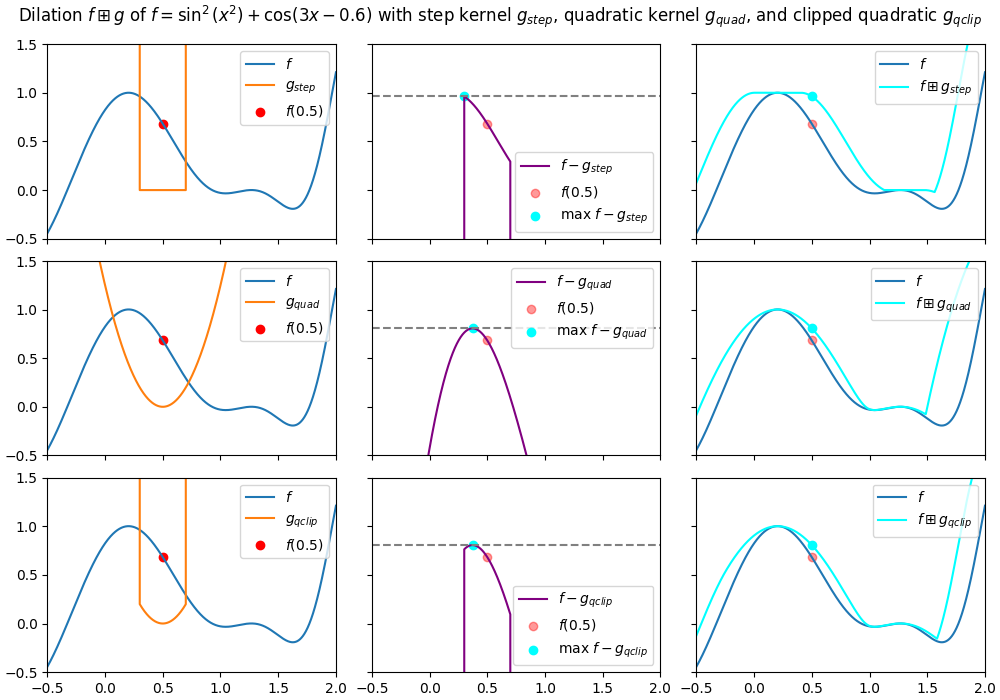
\includegraphics[width=\textwidth]{figures/dilation_illustration.png}
  \caption{Illustration of the effects of the dilation $\boxplus$ with three kernels on a sinusoidal $f$. $g_{step}=0$ in a region of size 0.5 and $-\infty$ outside, while $g_{quad}=-5x^2$ and $g_{qclip}=g_{quad}+g_{step}$. An alternative intuition for $\boxplus$ is also illustrated, corresponding with 'lowering' a negated version of $g'$ down towards the point $x$ until it intersects $f$ and taking the value of the lowered and flipped $g'(x)$ as the result of $\boxplus$ at point $x$. Note the continuous, thus lowercase $f$ and $g$.}
  \label{fig:dil-illust}
\end{figure}
\noindent
This result is interesting because we can see the standard max pooling layer in a convolutional neural network as a dilation with a fixed, step-function-like $G$ (a 2D version of $G_{step}$ from Fig. \ref{fig:dil-illust}). Generalising $G$ to be a quadratic form is a logical next step, where this thesis focuses on the anisotropic case.

In mathematical morphology, dilations and erosions come in pairs named adjunctions. It can be shown that the erosion which adjoins $\boxplus$, henceforth referred to as the operator $\boxminus$, is effectively a minimum weighted by a negated distance function \cite{heijmans1996morphological}: 
\begin{align}
	(F \boxminus G)[x]=\min_{y\in \mathcal{Y}}(F[x+y] - G[y])
\end{align}
\noindent
Using similar logic as above, we can show that, in the corresponding tropical min semifield\footnote{For both $T_+$ and $T_-$, it should be noted that standard addition $+$ is undefined for $\pm\infty$. In accordance with \cite{maragos}, we define $\forall x: x+(-\infty)=(-\infty)$ in $T_+$, while $\forall x: x+\infty=\infty$ in $T_-$} $T_-=(\mathbb{R}\cup\{\infty\},\min,+)$ \cite{maragos} with neutral elements $(\mathbb{0}=\infty, \mathbb{1}=0)$, the convolution with $\check{G}^*[y]=-G[-y]$ is equivalent to the erosion $\boxminus$ with $G$:
\begin{align}
	(F ~\textcircled{$*$}~ \check{G}^*)[x]
	&= \bigoplus_{y\in \mathcal{Y}}F[x-y] \otimes \check{G}^*[y] \\
	&= \min_{y\in \mathcal{Y}}(F[x-y] + \check{G}^*[y]) \\
	&= \min_{y\in \mathcal{Y}}(F[x-y] - G[-y]) \\
	\textrm{(Suppose $y^*=-y)$  }&= \min_{y^*\in \mathcal{Y}}(F[x+y^*] - G[y^*]) \\
	&= (F \boxminus G)[x]
\end{align}

\section{Further relevant mathematical morphology}
\label{sec:closing}
Aside from the common adjoint $(\boxplus,\; \boxminus)$ using $+$ and $-$ as the operators weighting each point, one can also define an adjoint that uses multiplication and division. This alternate adjoint on $\mathbb{R}_+$ then has the dilation $\dot \boxplus$, defined as \cite{heijmans1996morphological}:
\begin{align}
	(F~ \dot\boxplus~ G)[x] &= \bigvee_{y\in \mathcal{Y}}F[x-y]G[y]
\end{align}
However, it can be shown that this adjoint is equivalent (anamorphic) to the common adjoint $(\boxplus,\; \boxminus)$ using the transformation $t(x)=e^x$ and its inverse $t^{-1}(x)=\log(x)$. As such, using $\dot \boxplus$ would not result in a more expressive convolution while complicating implementation with the requirement of $\mathbb{R}_+$.

Two other concepts from mathematical morphology that do increase expressivity are the concepts of openings and closings \cite{heijmans1996morphological, gonzalez2017}. Here, an opening is an operator using an adjoint, where the input is first eroded and then dilated with the same structuring element $G$. Notably, an opening is anti-extensive (decreasing), meaning that for $(\boxplus,\; \boxminus)$ we can write the opening $\boxopen$:
\begin{align}
	\forall x\in\mathcal{Y}~~(F ~\boxopen~ G)[x] &= ((F\;\boxminus\; G)\;\boxplus\;G)[x] \leq F[x]
\intertext{
The operator dual to an opening is the closing using the same adjoint: here, a closing refers to first performing a dilation, and then performing the adjoining erosion with the same structuring element $G$. Notably, a closing is extensive (increasing), meaning that for $(\boxplus,\; \boxminus)$ we can write the closing $\boxclose$:
}
	\forall x\in\mathcal{Y}~~(F ~\boxclose~ G)[x] &= ((F\;\boxplus\; G)\;\boxminus\;G)[x] \geq F[x]
\end{align}
One of the possible advantages of using closings and openings over only dilations or erosions is that opening and closing both produce results with contours similar to their inputs \cite{gonzalez2017}. Illustrating the effects of the common opening and closing with a simple diagonal kernel in Figure \ref{fig:closing-illust}, we can see that the results of the closing have a higher value (due to the extensivity of $\boxclose$), but the shapes are less distorted by the shape of the kernel $G$ than the results of the dilation. 

This property, when combined with the extensivity of $\boxclose$, suggests it can also be used in the place of a dilation within the context of max-pooling for CNNs. As such, we will later apply the closing $\boxclose$ in that context, implemented as not a single semifield convolution \textcircled{$*$}, but a pair in $T_+$ and $T_-$ respectively.

\begin{figure}[hb!]
	\center
  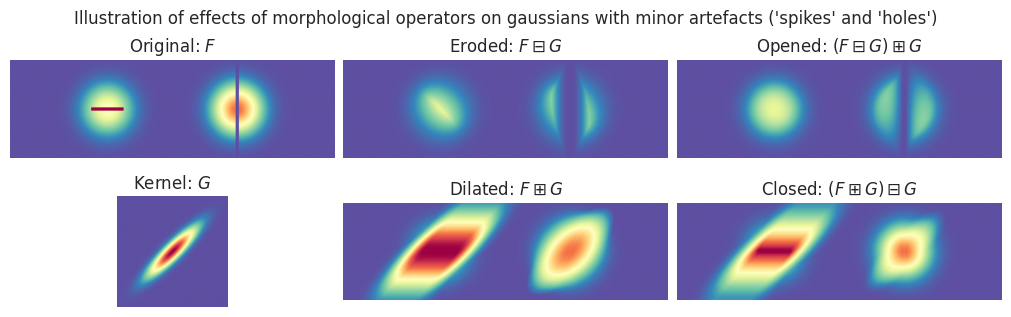
\includegraphics[width=\textwidth]{figures/closing.png}
  \caption{Illustration of the effects of opening and closing, where warmer (\textcolor{opening_red}{red}) colors  indicate higher values, and colder (\textcolor{opening_blue}{blue}) colors  indicate lower values.}
  \label{fig:closing-illust}
\end{figure}

\section{Variations of the convolution in CNNs}
Within a Convolutional Neural Network, there are layers typically referred to as convolutional layers. These layers apply an operator very similar to the discrete mathematical convolution $*$ of the input activations (or image) and a parameterised kernel (here with an explicit domain $\mathcal{X}$ for valid values of $x$):
\begin{align}
\forall x\in\mathcal{X}:~~(F*G)[x] &= \sum_{y\in\mathcal{Y}} F[x-y]\; G[y]
\end{align}
However, a CNN convolution has additional parameters that may change its behaviour. To better understand how we can apply semifield convolutions $\textcircled{$*$}$ in CNNs, we must therefore understand these parameters, usually named 'stride', 'dilation', 'padding'  and 'groups' in modern deep learning frameworks \cite{noauthor_conv2d_nodate, noauthor_xla_nodate}. Additionally, images and activations in CNNs have 'channels': an additional axis in the input, which is treated differently from the spatial ones. We will first discuss stride, dilation and padding, which do not interact with channels, and then discuss the concept of channels and convolutional groups.

Stride controls the spacing of the sampling grid for $F$ with respect to the output position $x$: where a regular convolution uses $F[x-y]$, a strided convolution would have $F[\textsc{stride}\times x - y]$. Striding can also be seen as 'moving' the receptive field (accessed values of $F$) of the convolution with a step size equal to the stride: see Fig. \ref{fig:stride-dilation-padding} for an illustration. For finite images, this reduces the size of the convolution result by shrinking the set of valid indices $\mathcal{X}$. Therefore, a $\textsc{stride}>1$ can allow later convolutions to be influenced by more inputs without increasing kernel sizes. A standard convolutional layer typically has a stride of 1, but a pooling layer might have a stride of 2 or higher.

Dilation is similar, but instead adjusts the step size for $y$: the term $F[x-y]$ becomes $F[x-\textsc{dilation}\times y]$, creating 'gaps' between the sampling points for $F$ (e.g.\ for $x=1$, sampling $F[-1]$, $F[1]$ and $F[3]$) without changing the sampling of the kernel $G$. However, a $\textsc{dilation}>1$ results in a locally non-smooth operator, which seems undesirable for smooth pooling. As such, none of the later experiments investigated using a $\textsc{dilation}>1$.

\begin{figure}[h!]
	\center
  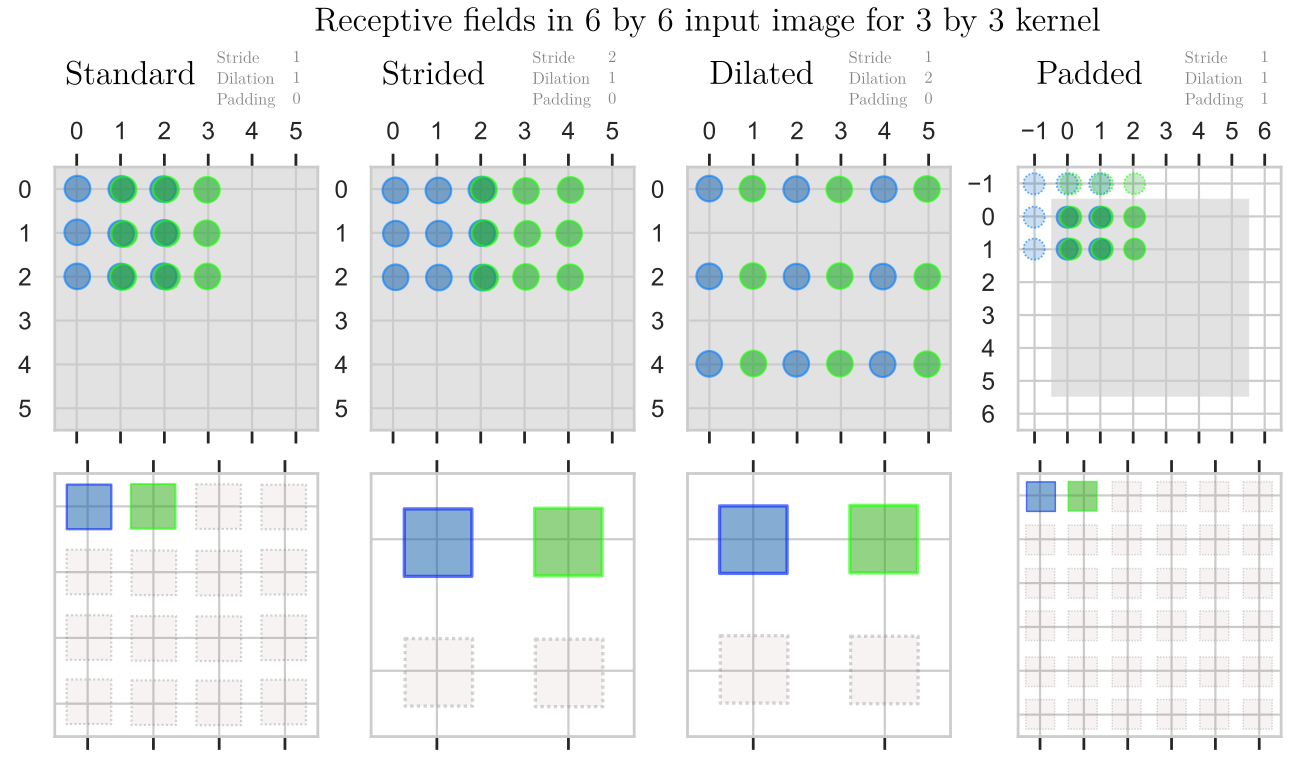
\includegraphics[width=0.87\textwidth]{figures/stride-dilation-padding.png}
  \caption{Illustration of the effects of stride, dilation and padding with a $3\times3$ kernel on a $6\times6$ input. The top row shows the receptive field of the reduction (accessed values of $F$), while the bottom row shows the output structure.}
  \label{fig:stride-dilation-padding}
\end{figure}

\noindent
Padding refers to convolving with a widened $F$: if a certain $F$ has domain $[0, 5]$, then a padding of 1 would correspond with convolving with an expanded $F'$ with domain $[-1, 6]$ that is equal to $F$ within $[0, 5]$. While there are many so-called border strategies \cite{gonzalez2017} in computer vision for how to determine the value of the newly added $F'[-1]$ and $F'[6]$, the method typically used within CNNs is to set these new values to be 0, thereby keeping the sum unchanged. 
Our use of padding lies in ensuring that the size of the output image does not shrink with kernel sizes larger than 1: this simplifies network structures by ensuring the output size decreases only if $\textsc{stride}>1$. For an odd-valued kernel dimensionality $K_o$ (such as $3\times3$, see Fig. \ref{fig:stride-dilation-padding}), this can be achieved by setting the padding to $\lfloor\frac{K_o}{2}\rfloor$. Even-valued kernel dimensionalities $K_e$ depend on where we define the centre of the kernel to lie. Suppose we define it as towards the lower indices in the kernel (up and to the left in 2D images) and allow for different amounts of padding at the beginning and end of $F$: in that case, we can retain image sizes by padding with $\frac{K_e}{2}-1$ at the low-index side of $F$ (top/left) and padding with $\frac{K_e}{2}$ at the high-index side of $F$ (bottom/right).


Aside from modifying the receptive field of the convolution, another way in which CNN convolutions can diverge from mathematical ones is in their use of a channel axis, distinct from the spatial axes. A small 2D RGB image might be stored as a $3\times50\times50$ array, but while the output index $x$ in a CNN convolution would represent a position in the X- and Y- axes of the image, the channel (colour) axis is not indexed. Instead, every convolutional kernel is responsible for one channel in the output and reads from a fixed set of channels in the input: while the kernel is 'moved' through the spatial dimensions during the convolution, it stays fixed relative to the channel dimensions. In a standard CNN convolution, all kernels read from all input channels, meaning that a square convolution of size 5 in this RGB image would require a convolutional kernel of size $3\times5\times5$ (as the kernel reads from 3 channels). In contrast, a typical max-pooling works per channel: every output channel only reads from one input channel. However, both cases can be seen as an adjusted version of the standard convolution formula. For a linear convolution, we simply add a summation over the set of input channels $\mathcal{C}$, indexing both $F$ and $G$ \cite{noauthor_conv2d_nodate}:

\begin{align}
\forall x\in\mathcal{X}:~~(F*G)[x] &= \sum_{c\in\mathcal{C}} \sum_{y\in\mathcal{Y}} F_c[x-y]\; G_c[y]
\end{align}
\noindent
Groups are then the parameter which allows us to precisely characterise this set of input channels $\mathcal{C}$. If the number of input- and output channels is a multiple of a certain number $N_{groups}$, then we can split both input and output into $N_{groups}$ equally sized groups. Here, $N_{groups}$ is the parameter named 'groups' in deep learning frameworks. A kernel in the $i$'th group of the output then reads from all the input channels in the $i$'th group of the input. For example, suppose we have an image with 6 input channels ($C_i=6$): $N_{groups}=1$ would result in every kernel reading from every input channel (a standard convolution), while $N_{groups}=C_i=6$ would make kernels read from only one channel (like a pooling). Values of $N_{groups}$ where $1<N_{groups}<C_i$ interpolate between these extremes, where every kernel reads a fixed subset of the input channels. It should be noted that while the number of output channels $C_o$ (equal to the number of kernels) is constrained to be a multiple of $N_{groups}$, the number of kernels per group in the output $S_o$ can be freely chosen and does not need to equal the number of channels per input group $S_i$: see Fig. \ref{fig:channels-groups} for examples.

\begin{figure}[h!]
	\center
  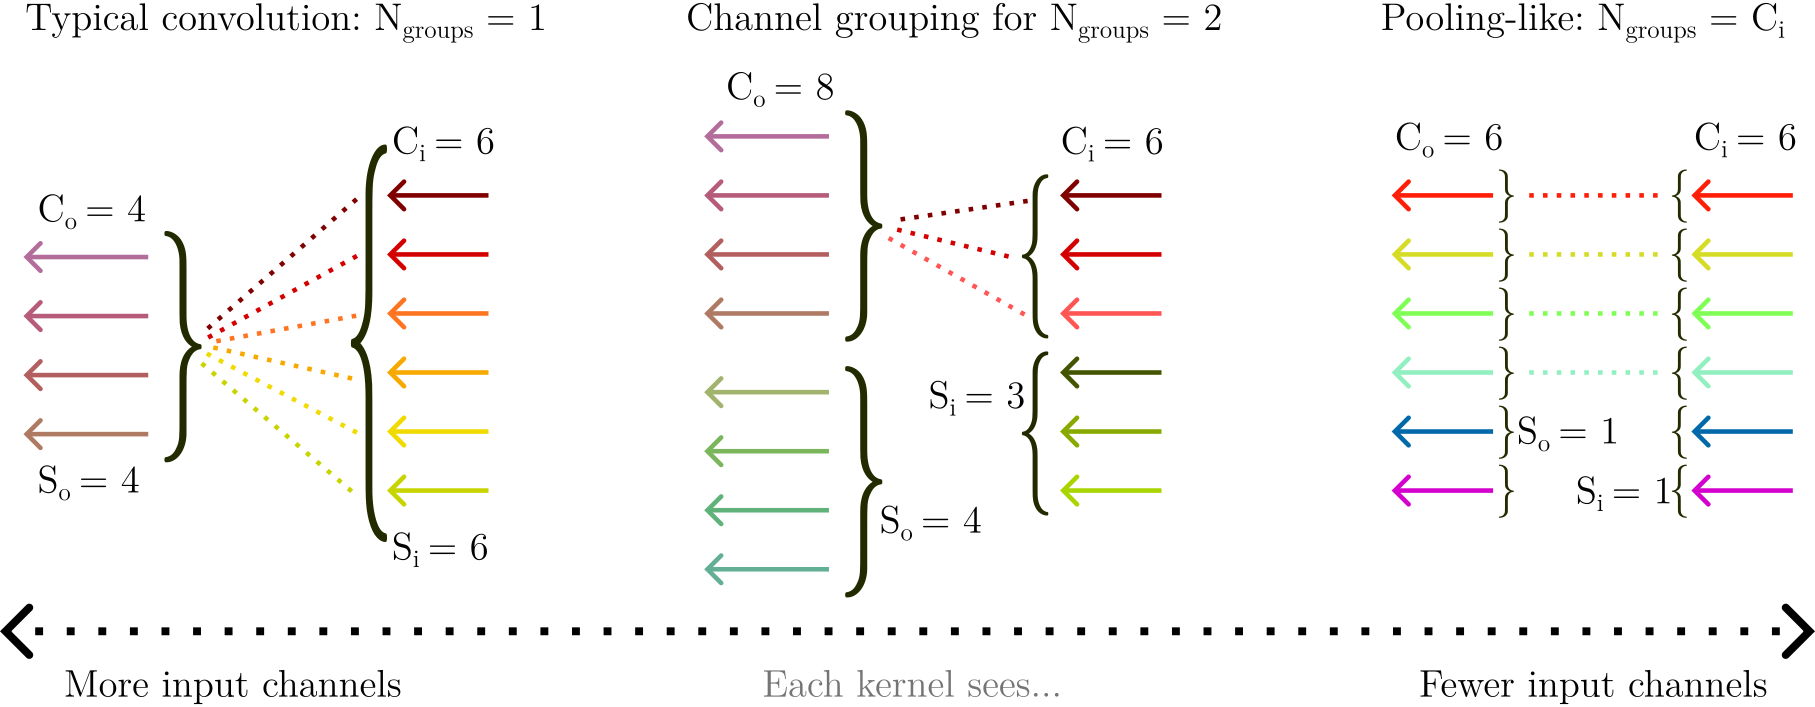
\includegraphics[width=\textwidth]{figures/channels-groups.png}
  \caption{Illustration of channels in the input and output, and the effects of the group parameter on which input channels are read by the kernels.}
  \label{fig:channels-groups}
\end{figure}

\section{Non-morphological semifields}
\label{sec:non-morph}
In previous sections, we discussed two semifields related to mathematical morphology, namely $T_+$ and $T_-$, and showed their correspondence with the pooling layers within a CNN. Using these results, we could see that a max-pooling was equivalent to a semifield convolution (in $T_+$, with a flat kernel). However, the linear convolutional layers within a CNN can also be interpreted as a semifield convolution in the corresponding linear semifield
$L=(\mathbb{R}, +, \times)$: filling in the equation for $\textcircled{$*$}_L$ (Eq. \ref{eq:semifield-conv}), we would again obtain a standard convolution $*$.

This raises the question of whether there are alternative semifields that act similarly to the linear semifield, such that they could be used in place of the standard convolutional layer in a CNN. In an investigation of some semifields, \cite{bellaardaxiomatic} identified sets of relevant semifields that were isomorphic (equivalent under a bijective mapping) to the linear semifield $L$. These can be written as:

\begin{itemize}
	\item[$L_{\mu+}$]  The positive log semifields:  $(\mathbb{R}\cup \{-\infty\}, \oplus_\mu, +)$ for all $\mu>0$ where \\$a\oplus_\mu b= \frac{1}{\mu}\ln(e^{\mu a}+e^{\mu b})$, $\mathbb{0}=-\infty$ and $\mathbb{1}=0$ 
	\\(with $\forall x\;e^{x+(-\infty)}=e^{-\infty}=0$)
	\item[$L_{\mu-}$]  \gray{The}\ negative \gray{log semifields:\  $(\mathbb{R}\cup \{{\color{black}+\infty}\}, \oplus_\mu, +)$ for all ${\color{black}\mu<0}$ where \\$a\oplus_\mu b= \frac{1}{\mu}\ln(e^{\mu a}+e^{\mu b})$, $\mathbb{0}={\color{black}+\infty}$ and $\mathbb{1}=0$}
	\item[$R_p$]  The root semifields:  $(\mathbb{R}_+, \oplus_p, \times)$ for all $p\ne0$ where \\$a\oplus_p b= \sqrt[p]{a^p+b^p}$, $\mathbb{0}=0$ and $\mathbb{1}=1$
\end{itemize}

\noindent
In \cite{bellaardaxiomatic} it was also noted that the positive log semifield $L_{\mu+}$ becomes equivalent to $T_+$ when $\mu$ approaches $+\infty$, while $L_{\mu-}$ becomes equivalent to $T_-$ as $\mu$ approaches $-\infty$. 
Additionally, one can see that the root semifields $R_p$ also become equivalent to $T_+$ when $p$ approaches $+\infty$, as $\oplus_p$ then becomes the infinity-norm (which is equivalent to $\max$). Informally, the reader may also convince themselves that as $p$ approaches $-\infty$, the semifield addition $\oplus_p$ approximates $\min$, making a theoretical $R_{-\infty}$ equivalent to $T_-$ (out of scope for this report).

These additional equivalences with $T_+$ suggest the possibility of using log or root semifields with high values for $\mu$ or $p$ as another alternative for traditional max-pooling layers in CNNs. It should be noted, however, that neither log nor root semifields seem to be part of an adjoint, meaning the resulting pooling would likely not be easily modelled using principles of mathematical morphology, and many of the theoretical guarantees might be lost.

% $\sqrt[\infty]{\frac{1}{\frac{1}{a^\infty}+\frac{1}{b^\infty}}}$

\chapter{Method}
With a greater understanding of semifields, convolutions, and some relevant examples of semifield convolutions, we can now examine how to apply semifield convolutions within the context of CNNs. 
First, we will review some implementation notes on semifield convolutions and describe how to use quadratic forms to parameterise convolutional kernels. Afterwards, we will describe the experimental setup used to examine which quadratic forms work best in the context of CNNs and which parameters of a semifield convolution positively impact a CNN's performance on various image classification tasks.



\section{Semifield convolutions in a CNN}

Previous sections described the theory underlying a semifield convolution and the additional parameters available in a CNN, but applying this in practice requires an efficient implementation. For this purpose, we wrote two packages: \verb pytorch-semifield-conv , which uses Just-In-Time (JIT) compilation to create convolutional operators, and \verb pytorch-numba-extension-jit , which automatically generates C++ bindings for the operators and aids in the JIT compilation process. More details on these packages can be found in the Extension report \cite{extension} and the documentation of the packages. For a simple verification of the learnability of the kernel parameters, see Appendix \ref{sec:poc}.

While implementation details will be left to the Extension report, two notable differences exist between the semifield convolutions used in this report and the descriptions of similar operators in previous works \cite{thierrybsc, koenbsc}. 

Firstly, the dilations used for this report do not spread the gradient between multiple maxima (i.e.\ if there are two equal maxima, assign both a gradient of 0.5 instead of picking one to have a 1.0 gradient). This spreading is the behaviour of the \verb torch.amax  function, but \verb torch.max  is more efficient and does not spread the gradient. Similarly, the CUDA kernels created for this report also do not spread the gradient. Some small-scale experiments were done to investigate whether spreading the gradient has a meaningful impact, but these showed no difference (as equal maxima are exceedingly rare \cite{thierrybsc}).

Secondly, summation across channels is always done using semifield addition. For dilations, some have proposed using scalar addition instead of the maximum across channels \cite{koenbsc, fan2021alternative}. However, various small-scale experiments consistently showed slightly worse performance for quadratic kernels when replacing $\max$ with $+$ across channels. Since this report focuses solely on quadratic kernels, this modification was not considered during the experiments.



\newpage
\section{Generating dilation kernels with quadratics}
For a standard linear convolution, we typically use a fully learned kernel. Since the reduction operation in the linear semifield is $+$, the partial derivative of the summation result is equal to a constant $1$ for all terms, and all parts of the kernel can typically receive a portion of the gradient during backpropagation.

However, this is not the case for dilations; a convolution in $T_+$ uses $\max$ as the reduction operator, meaning that only one term receives a non-zero gradient. If the kernel were fully parameterised (every value learned separately), fitting the kernel would be very challenging due to the overly sparse gradient. As such, we can instead choose to generate a kernel based on a parameterised function, reducing the number of parameters to be learned by gradient descent.

There are many options for generating a kernel-like array, but the context of replacing a max-pool with dilation can help suggest reasonable constraints. Firstly, the result of a max-pool can never be below the original value; in a dilation, we can ensure this by setting the centre of the kernel to $0$. Secondly, the result of a max-pool is, at most, the maximum value in an area and never higher; we can ensure this by using a nonpositive kernel: $\forall y,~G[y] \leq 0$. Finally, we may consider it reasonable for the kernel to be concave, as this ensures spatial locality (we cannot 'skip over' a pixel when looking for the maximum).


Combining these requirements, we can see that an alternative formulation for such a kernel function would be a function that evaluates the distance to the centre of the kernel for all points and uses the negative of that distance for the value of the kernel $G$. Formally, such a kernel function can be viewed as a metric (see \cite{metrics}) $d$ on the space of kernel indices $\mathcal{I}$, with the values at any point $\mathbf{y}\in\mathcal{I}$ in the kernel being the negated distance to the kernel centre $c_k$:
\begin{align}
	\forall \mathbf y,~~G[\mathbf y]=-d(\mathbf y, c_k)
\end{align}
Using this formalism, we see that all appropriate kernel functions derive from metrics calculating a 2D distance. If we further set $c_k$ to be the origin of $\mathcal{I}$, we can write any distance function as $d(\mathbf y)$ (with the centre implicit, effectively equivalent to a vector norm). A straightforward distance we could choose might be the squared distance to the origin $d(\mathbf y)=\mathbf y^T\mathbf y$, but this is nonparametric. Adding a parameter could then lead to the isotropic quadratic:
\begin{align}
	\textrm{Isotropic quadratic kernel: }&G[\mathbf y] = -\mathbf y^T(sI)^{-1}\mathbf y
\intertext{
Here, the scalar $s$ can be adjusted to control how quickly the distance rises and the kernel values fall. However, the isotropic quadratic only generates kernels where the contour lines are circles. To allow for non-circular kernels, we must allow dimensions to be weighted differently. A candidate function could then be the anisotropic quadratic (the Mahalanobis distance to the origin):
}
	\textrm{Anisotropic quadratic kernel: }&G[\mathbf y] = -\mathbf y^T\Sigma^{-1}\mathbf y
\end{align}
By learning a $2\times2$ positive definite matrix for $\Sigma$, we can then parameterise a kernel function for a 2D dilation kernel $G$ with elliptical contour lines. Testing whether moving from circular contours to elliptical contours improves CNN performance is the primary subject of this report and later experiments.

Finally, it should be noted that the choice of these quadratic kernels is not arbitrary. When used for dilations, these 'quadratic forms' have theoretical advantages regarding smoothness and rotational symmetry, similar to how kernels based on their exponentiation (the Gaussian) act in linear convolutions.

\newpage
\section{Learning quadratic kernel parameters}
\label{sec:learning-pdm}
In order to apply the aforementioned quadratic kernels in a neural network, we must first devise a parameterisation scheme that can be used for gradient-based optimisation. For both types of quadratic kernels, the equivalent of the Mahanalobis distance covariance matrix ($sI$ for isotropic, $\Sigma$ for anisotropic) must be positive definite. With an isotropic kernel, using a parameter $\theta$ where $\theta = \log s$ ensures that $s$ is positive, and thus that $sI$ is positive definite. However, the matrix $\Sigma$ for the anisotropic case requires more care. If the entire matrix were freely learned via gradient descent, an optimisation step may result in $\Sigma$ no longer being positive definite, violating the kernel requirements.

One method for resolving this involves viewing $\Sigma$ as a $2\times2$ covariance matrix and parameterising it accordingly. Since $\Sigma$ must, in that case, be symmetric, we know by the spectral theorem that $\Sigma$ is diagonalisable \cite{poole2015linear}:
\begin{align}
\textrm{For some orthogonal matrix }Q &\in \mathbb{R}^{2\times 2} \textrm{, and} \nonumber \\
\textrm{for some diagonal matrix }D &\in \mathbb{R}^{2\times 2} \textrm{,}\nonumber \\
\Sigma &= QDQ^T\\
&= Q \begin{bmatrix}
	 \sigma_1^2 & 0\\ 0 &  \sigma_2^2
\end{bmatrix} Q^T
\end{align}
Here, Q (as an orthogonal matrix) can either be a rotation or a reflection. However, since $Q$ occurs twice, its determinant cancels, and fixing $Q$ to be a rotation does not reduce expressivity (see Appendix \ref{sec:red-mirr}). As such, we can use:
\begin{align}
\Sigma = \begin{bmatrix}
	\cos \phi & -\sin \phi \\ \sin\phi & \cos\phi
\end{bmatrix}\begin{bmatrix}
	 \sigma_1^2 & 0\\ 0 &  \sigma_2^2
\end{bmatrix} \begin{bmatrix}
	\cos \phi & \sin \phi \\ -\sin\phi & \cos\phi
\end{bmatrix}
\end{align}
This parameterisation can be efficiently inversed for the quadratic form, as \begin{align}
	\Sigma^{-1} &= (QDQ^T)^{-1}\\
	&= (Q^T)^{-1} D^{-1} Q^{-1}\\
	&= Q\begin{bmatrix}
	 \frac{1}{\sigma_1^2} & 0\\ 0 &  \frac{1}{\sigma_2^2}
\end{bmatrix}Q^T
\end{align}
In order for $\Sigma$ to be positive-definite, $\sigma_1^2$ and $\sigma_2^2$ are required to be strictly positive, while there are no constraints on $\phi$. As such, for any $\boldsymbol{\theta}\in\mathbb{R}^3$:
\begin{align}
\textrm{Let }\boldsymbol{\theta}&=\begin{bmatrix}
	\theta_1\\
	\theta_2\\
	\theta_3\\
\end{bmatrix}=\begin{bmatrix}
	\log|\sigma_1| \\
	\log|\sigma_2|\\
	\phi\\
\end{bmatrix}, \textrm{ then a valid $\Sigma^{-1}$ would be} \\
\Sigma^{-1} &= \begin{bmatrix}
	\cos \theta_3 & -\sin \theta_3 \\ \sin\theta_3 & \cos\theta_3
\end{bmatrix}\begin{bmatrix}
	 e^{-2\theta_1} & 0\\ 0 &  e^{-2\theta_2}
\end{bmatrix} \begin{bmatrix}
	\cos \theta_3 & \sin \theta_3 \\ -\sin\theta_3 & \cos\theta_3
\end{bmatrix}
\end{align}
Since we placed no assumptions on $\boldsymbol{\theta}$, it is safe for a black-box or gradient-based optimiser to adjust in any direction, as the resulting $\Sigma$ will always be a positive definite matrix. As such, this is an appropriate parameterisation for the matrix $\Sigma$ in an anisotropic quadratic kernel.

This parameterisation further has the advantage of being easily interpretable: $e^{\theta_1}$ and $e^{\theta_2}$ are equivalent to the standard deviations of a hypothetical 2D multivariate normal distribution with contours of the same shape as the quadratic kernel, while $\theta_3$ is the counter-clockwise angle the first principal axis forms with the x-axis. An alternative parameterisation for a covariance matrix $\Sigma$, based on the Pearson correlation coefficient, can be found in Appendix \ref{sec:pearson}.




\newpage
\section{Initialising quadratic kernel parameters}

While we now have definitions for appropriate parameters $\boldsymbol{\theta}$ that can be used for quadratic kernels, we must determine how to initialise these parameters.

One straightforward approach would be to use uniform-random or Gaussian initialisation. However, previous work has shown that initialising kernels such that different possibilities are explored can aid in the learning process \cite{thierrybsc}.

For the initialisation of the isotropic scale\footnote{Blankenstein, like \cite{groenendijk2022morphpool}, used $s$ scaled up by 4, having $-\frac{1}{4s}\mathbf{y}^T\mathbf{y}$ as the isotropic quadratic (despite claiming otherwise in their report and comments, their implementation is as such). } $s$, \cite{thierrybsc} suggested using evenly spaced\footnote{Linearly spaced, i.e.\ interpolated between the endpoints at $\frac{i}{\textsc{n-kernels-1}}$ for kernel $i$.\\While examining Fig. \ref{fig:init} might suggest that a log-scale may be more appropriate, small-scale experiments show a consistent decrease in performance when using logarithmic spacing.  } scales between $s=1$ (where only the centre of the kernel is $>-1$) and $s=2~\lfloor\textsc{kernel-size}/2\rfloor^2$ (where only the corners are $\leq-1$). Supposing the images are normalised to the range $[0, 1]$, this approach would ensure that all relevant kernel sizes are represented after initialisation (see Fig. \ref{fig:init}, top row).

For initialising anisotropic kernels, we consider two methods. The first method initialises the variances of the kernel isotropically in the same manner as before: this has the advantage of strengthening the idea of anisotropic kernels being 'no worse than isotropic', as they would begin isotropically. The alternative approach involves initialising the variances heavily skewed: one axis with low variance and one with high variance. In the experiments, this is done by sampling variances uniform randomly from $[1, 8]$ and $[20, 24]$, respectively. When combining this with evenly spaced\footnote{Linearly spaced \textit{without the final value}, i.e.\ interpolated at $\frac{i}{\textsc{n-kernels}}$ for kernel $i$.
\\
This skips the last orientation, as $\theta=\pi$ would be equivalent to $\theta=0$ for these kernels. \vspace{-0.25cm}
} angles $\theta\in[0, \pi)$, we can create kernels that lift the input to an orientation score (like \cite{smetspde}). While a scale space would aid in learning features at various scales, this 'orientation space' might aid in learning to recognise lines and edges. For a visualisation, see Fig. \ref{fig:init}:

\begin{figure}[b!]
	\center
  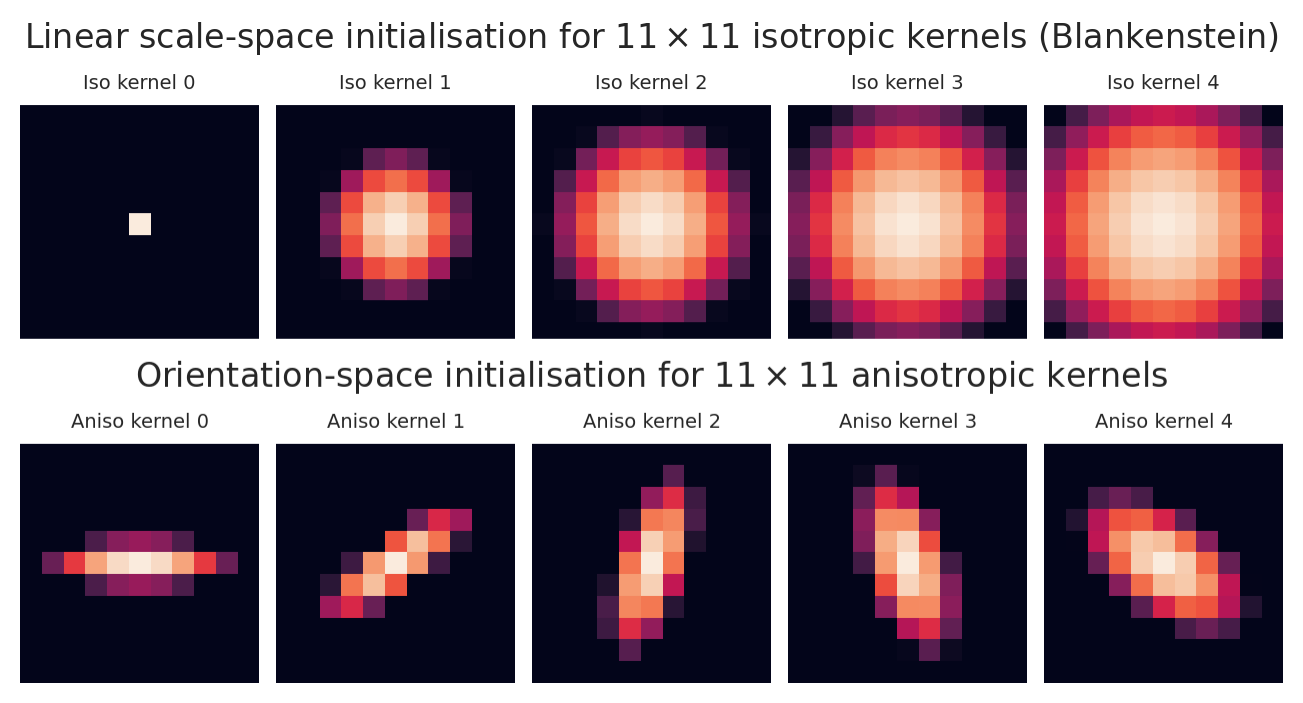
\includegraphics[width=\textwidth]{figures/initialisation.png}
  \caption{Initialisation of five $11\times11$ kernels: here, isotropic kernels (top) are initialised with a linear scale-space \cite{thierrybsc}, while anisotropic kernels (bottom) are initialised with skewed variances and evenly spaced angles  $\theta \in [0, \pi)$. In the images, black is a value  $\leq-1$, while white is 0. In practice, kernels are shuffled to prevent bias (occurs when followed by a layer with $\textsc{groups}\neq1$)}
  \label{fig:init}
\end{figure}

\newpage
\section{Classification datasets and models}
To determine the effects of isotropic and anisotropic dilations as a replacement for max-pooling, we must decide on a measure of performance. Keeping in line with previous experiments on this topic \cite{groenendijk2022morphpool, thierrybsc, koenbsc}, we will be evaluating the performance of image classification models on (relatively small) image datasets, with test-set accuracy as the primary metric.
The datasets used are:
\begin{itemize}
\setlength{\itemsep}{0pt}
	\item K-MNIST: grayscale, 10 classes, each a cursive Japanese character \cite{k-mnist}. 
	\item Fashion-MNIST: grayscale, 10 classes, each a fashion item \cite{fashion-mnist}.
	\item CIFAR10: RGB, 10 classes, containing various real-world objects \cite{cifar10}.
	\item SVHN:  RGB, 10 classes, each a digit as seen in a house number \cite{svhn}.
\end{itemize}
The model architecture for the first two datasets is LeNet-5 \cite{lenet5}, just as in previous research \cite{thierrybsc}.
The other two datasets use a typical CNN, taken from \cite{model-cifar}.
For a visualisation of the datasets and the models, see Fig. \ref{fig:datasets}:
\begin{figure}[h!]
	\center
  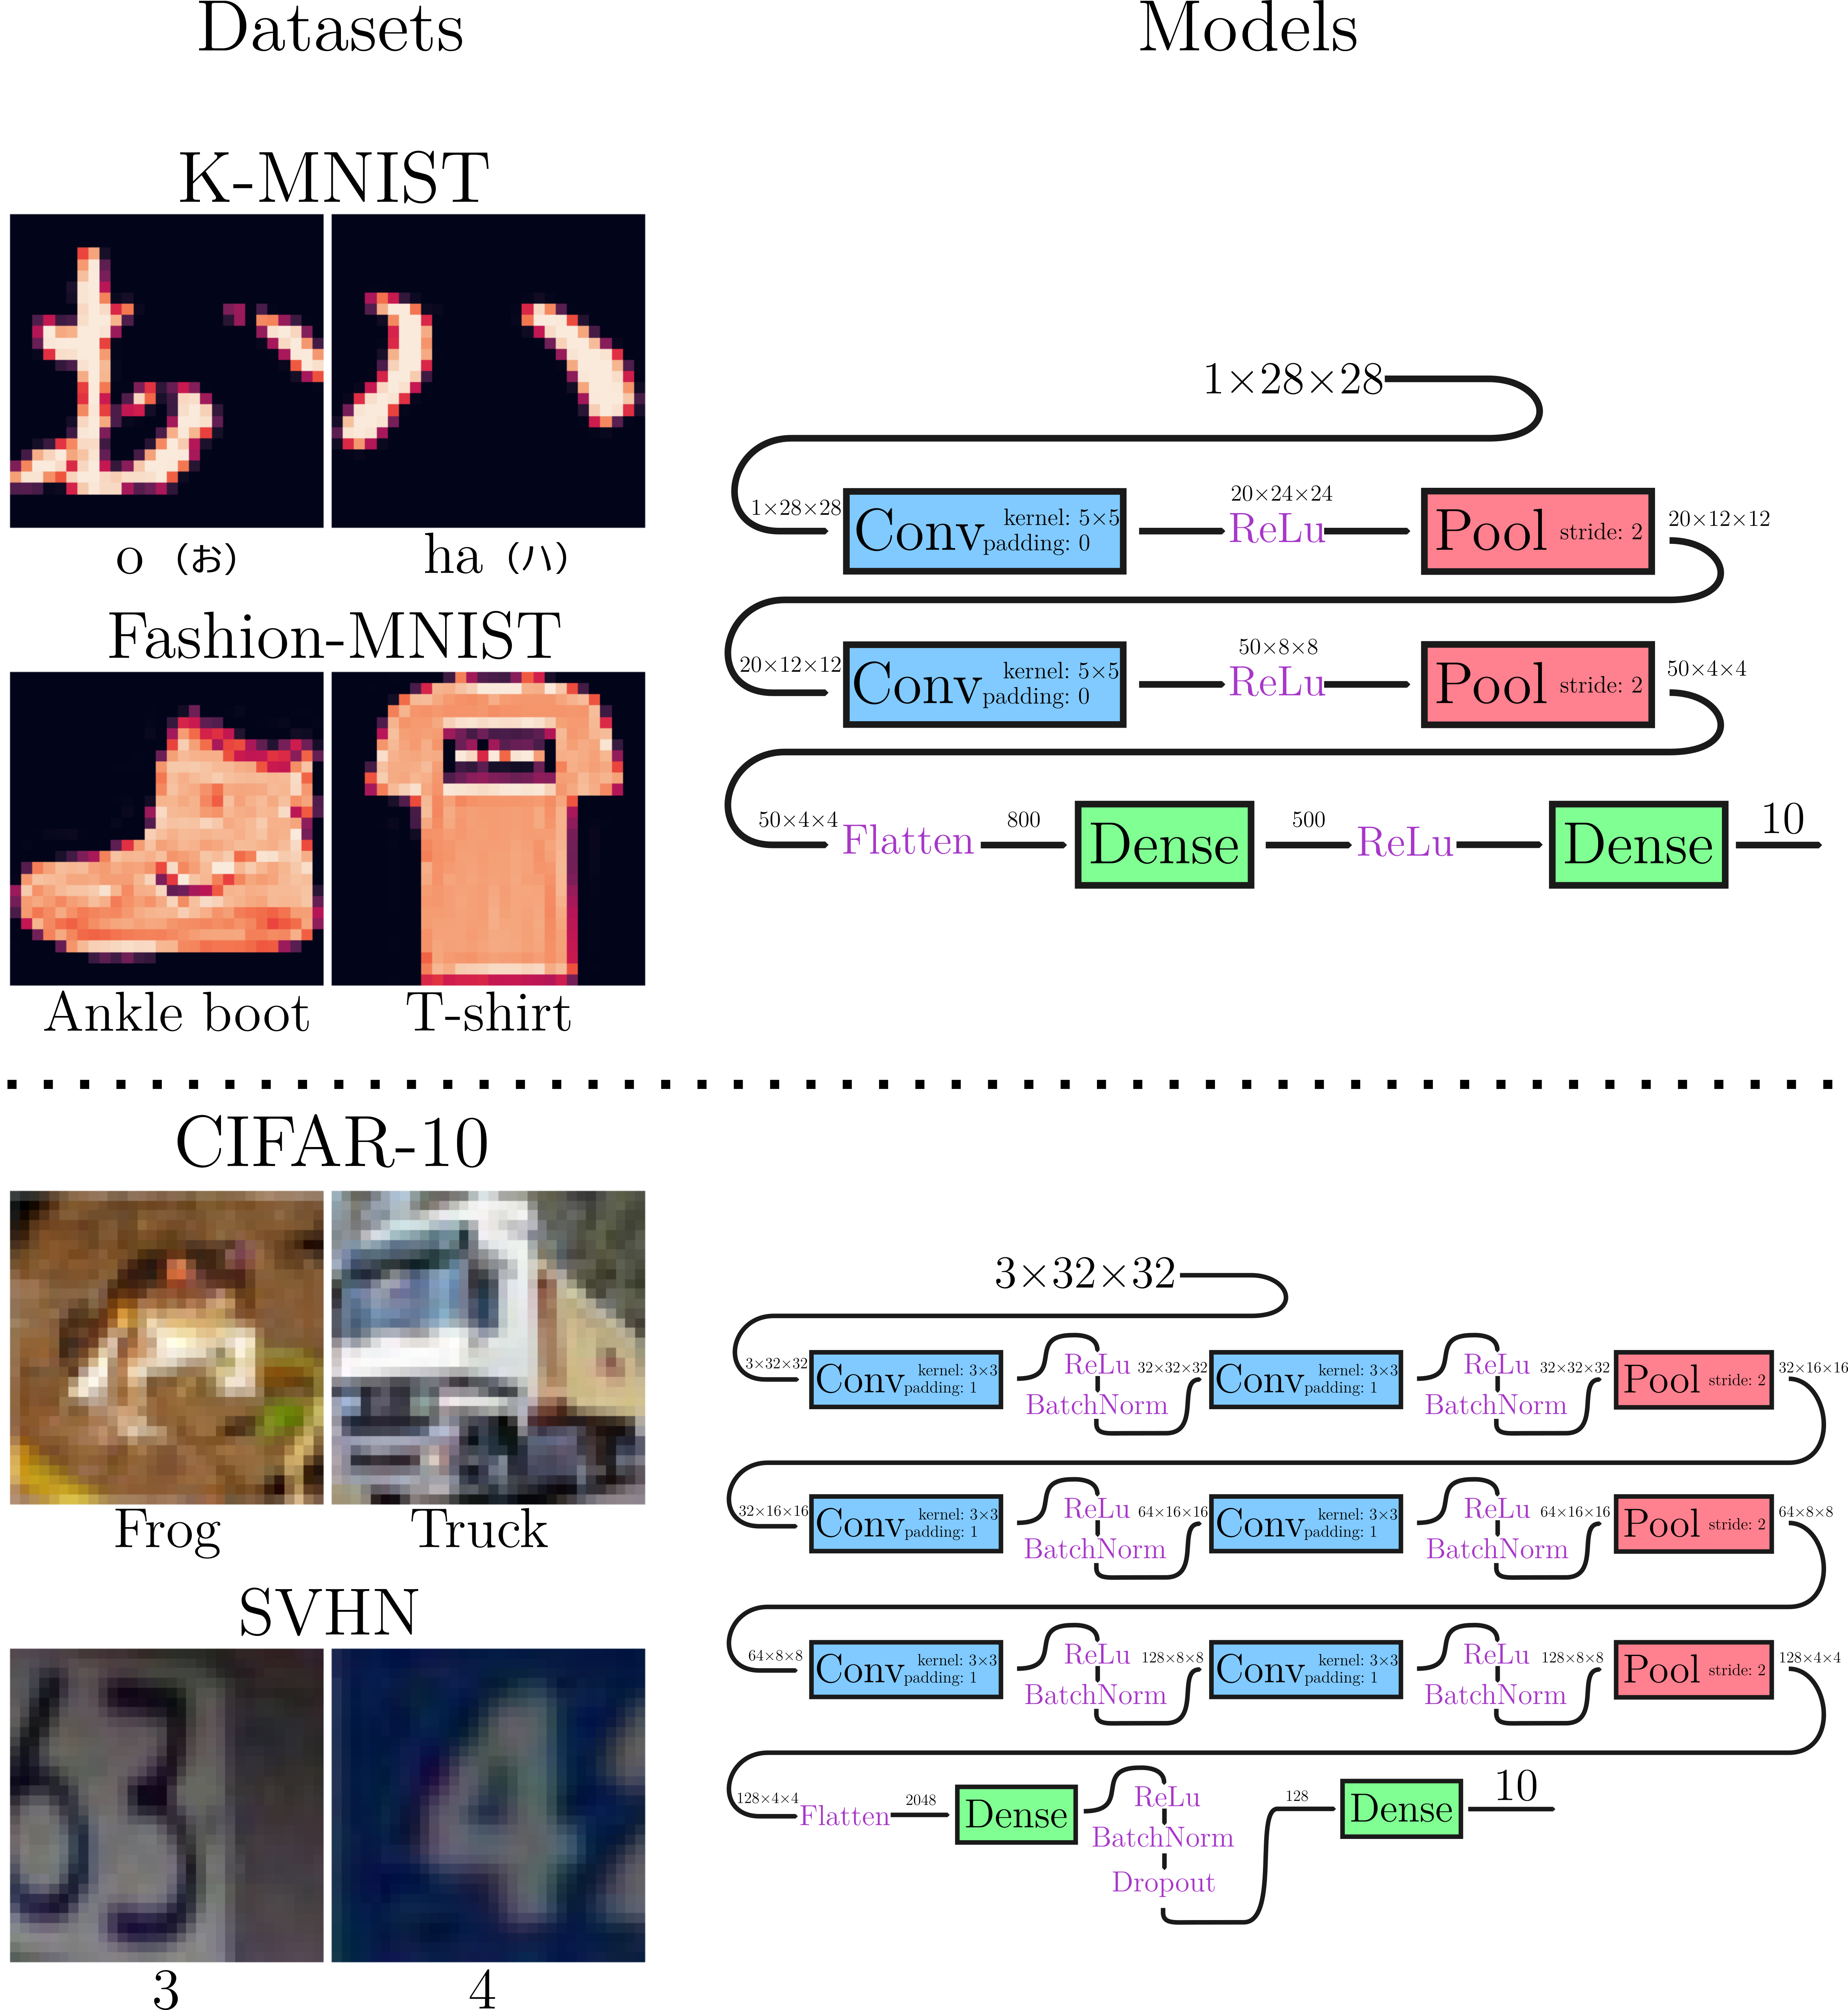
\includegraphics[width=1\textwidth]{figures/datasets.png}
  \caption{Illustration of datasets and models used for experimentation.
  The pooling layers are left generic: specific kinds of pooling will be discussed next. }
  \label{fig:datasets}
\end{figure}

\newpage
\section{Experimental setup}
\label{sec:setup}
Both models shown in Fig. \ref{fig:datasets} have a placeholder for the specific kind of pooling, as this will be the hyperparameter we vary during the experiments.
For the main set of experiments: the following kinds of poolings will be used:
\begin{itemize}
\vspace{-0.1cm}
\setlength{\itemsep}{0pt}
	\item \textbf{Standard}: a typical max-pooling, with kernel sizes\footnote{A pooling of kernel size 1 is equivalent to subsampling the image, and serves as a baseline} between 1 and 5
	\item \textbf{Isotropic}: a dilation with an isotropic kernel, with kernel sizes 2, 3, 5, 7 and 11 and initialised using scale-space initialisation.
	\item \textbf{Anisotropic}: a dilation with an anisotropic kernel, with kernel sizes 2, 3, 5, 7 and 11. Initialisation will be one of scale-space or orientation-space.
\end{itemize}
\vspace{-0.1cm}
Afterwards, a secondary set of experiments will be run to examine the effects of the \textsc{groups} parameter for poolings and the usage of closings $\boxclose$. The best kernel size from the main set will be reused for these experiments.

The secondary set of experiments will use the following kinds of poolings:
\begin{itemize}
\vspace{-0.1cm}
\setlength{\itemsep}{0pt}
	\item \textbf{Iso-grouped} / \textbf{Aniso-grouped}: Same as \textbf{Isotropic} / \textbf{Anisotropic}, but now with $\textsc{groups}=\frac{\textsc{channels}}{2}$, such that each layer sees two channels.
	\item \textbf{Iso-closing} / \textbf{Aniso-closing}: Same as \textbf{Isotropic} / \textbf{Anisotropic}, but now with a morphological closing $\boxclose$ instead of a dilation $\boxplus$ (see Sec. \ref{sec:closing})
\end{itemize}
\vspace{-0.1cm}
Finally, some exploratory experiments were run to investigate the effects of using non-linear semifields for standard convolutions (see Sec. \ref{sec:non-morph}). Appendix \ref{sec:nonlinconv} describes these extra experiments and their results.

Since the pooling layer is the only hyperparameter we wish to vary during experiments, we must fix all others. While extensive hyperparameter tuning was not considered necessary for this report, various learning rates were examined across epochs to determine a representative set of hyperparameters (see Appendix \ref{sec:hyperparameters}). The chosen hyperparameters are displayed in Table \ref{table:hyperparameters}:

\begin{table}[!htbp]
\centering
\begin{tabular}{l|*4c}
\toprule
Hyperparameter & K-MNIST & Fashion-MNIST & CIFAR-10 & SVHN\\
\midrule
Batch size & \multicolumn{4}{c}{1024 (saturates GPU compute)}\\
Optimiser   &  \multicolumn{4}{c}{Adam, default parameters except \textsc{lr}} \\
Learning rate & 0.004 & 0.003 & 0.004 & 0.003 \\
Epochs & 30 & 80 & 150 & 250 \\
\bottomrule
\end{tabular}
\caption{Hyperparameters used when training models on datasets.}
\label{table:hyperparameters}
\end{table}
\noindent
All experiments were run on one machine, with the final results being generated using the following hardware and versions of software:

\begin{table}[!htbp]
\centering
\begin{tabular}{l|c}
\toprule
Component & Name \\
\midrule
CPU & Intel i9-13900K \\
GPU & NVIDIA RTX 5090 \\
CUDA & 12.8\\
OS & Ubuntu 24.04.2\\
\bottomrule
\end{tabular}
\quad
\begin{tabular}{l|c}
\toprule
Software & Version \\
\midrule
Python & 3.12.9 \\
PyTorch & 2.7.0+cu128 \\
TorchVision & 0.22.0+cu128 \\
\small pytorch-semifield-conv & \comment{0.2.0?} \\
\bottomrule
\end{tabular}

\caption{Hardware and software used for the experiments. The package \textsc{pytorch-semifield-conv} is described in the Extension report \cite{extension}.}
\vspace{-0.3cm}
\end{table}


\chapter{Results}
\label{sec:results}
As described in Sec. \ref{sec:setup}, the experiments performed involve testing variations of pooling layers using the models and datasets shown in Fig. \ref{fig:datasets} (experiments with $R_p$ and $L_\mu+$ can be found in Appendix \ref{sec:nonlinconv}).
To obtain reliable results, every model configuration was trained repeatedly (100 times for K-MNIST and Fashion-MNIST, 40 times for CIFAR-10 and SVHN), and the results were aggregated. The primary metric that model configurations will be compared on is the mean test-set accuracy, while confidence intervals denoting the 5th and 95th percentiles\footnote{Using percentile-based confidence intervals deviates from previous work \cite{thierrybsc, koenbsc}, which used one standard deviation. This is intentional, as some unstable configurations might occasionally produce low-accuracy (e.g.\ 50\% or 70\%) results. Under the Gaussian assumption of standard deviations, this uncertainty would be modelled symmetrically, and the top of the error bar would be drawn overly high (above the highest observed value, at times).} of accuracy scores are displayed for context.

The format of graphs in this chapter is such that all results are grouped per kernel type (standard/non-dilation, isotropic, anisotropic with scale-space initialisation or anisotropic with orientation-space initialisation), with a secondary hyperparameter being varied within the group. Within each group (kernel-kind), the best-performing configuration is highlighted, and the values for these best-performing configurations are repeated for comparison at the right of each subplot (above 'Best'). Note that most plots are zoomed in such that the total height is \textbf{two percentage points}: differences are minor.

\section{K-MNIST and Fashion-MNIST}
Examining Fig. \ref{fig:res-small}, we can see that swapping the standard pooling layer for a dilation consistently improves performance for a LeNet-5 on K-MNIST. Anisotropic kernels outperform isotropic kernels, with both methods for initialisation attaining similar peak results for $11\times11$ kernels and somewhat differing results for the other kernel sizes.

However, the situation changes considerably when we examine model performance on Fashion-MNIST. Here, the standard max-poolings consistently outperform dilations, with only a $3\times3$ orientation-space anisotropic kernel approaching the performance of a standard max-pooling. These results are consistent across runs, but the cause is unclear. Two possible explanations are that a larger model would be required to effectively use dilation-based poolings and/or that the images from Fashion-MNIST are poorly suited for dilations. 

Notably, all pooling types remain better than subsampling ($1\times1$ pooling).


\newpage
\begin{figure}[ht!]
	\center
  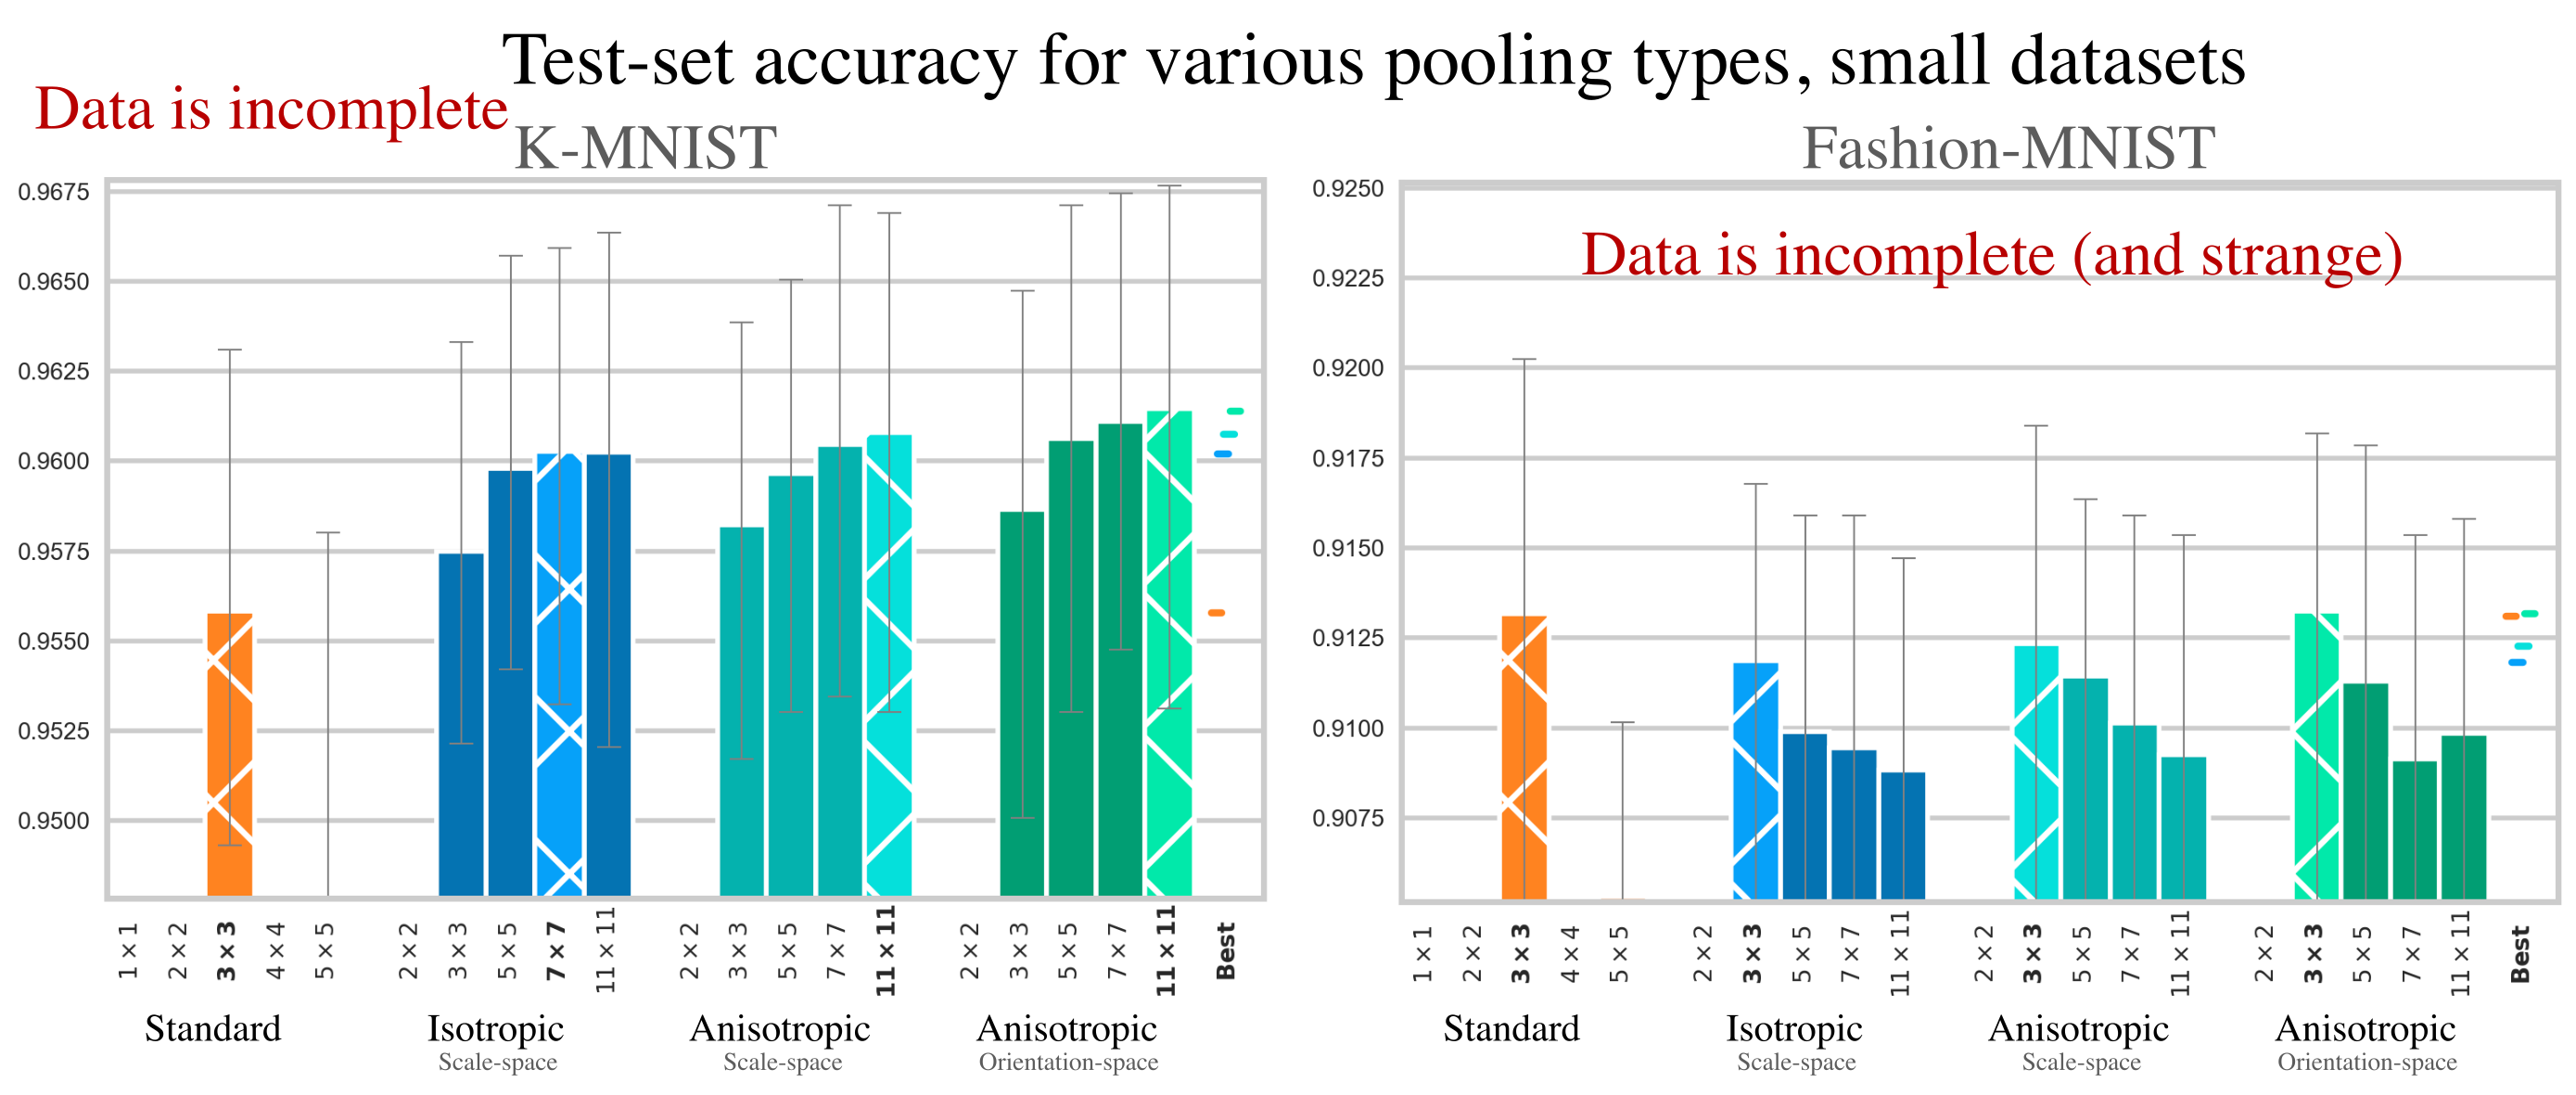
\includegraphics[width=1\textwidth]{figures/results-small.png}
  \caption{Accuracy (mean of 100) for model configurations on small datasets}
  \label{fig:res-small}
\end{figure}

\vspace{-0.7cm}
\section{CIFAR-10 and SVHN}
In Fig. \ref{fig:res-large}, we can see that the best kernel sizes for dilations outperform standard max-pooling layers for both datasets. For CIFAR-10, dilations outperform max-poolings at all kernel sizes save $2\times2$, with anisotropic kernels slightly outperforming the correspondingly sized isotropic kernels. When training on SVHN, we can see that standard max-poolings are better up to $5\times5$ kernels, whereafter dilations take the lead. Additionally, though anisotropic poolings scale similarly with kernel size to isotropic poolings, it appears as if anisotropic poolings perform slightly worse than their isotropic counterparts.

%It appears as if anisotropic dilations are slightly worse than isotropic dilations for both initialisation types, though the scaling with kernel size shows the same pattern.

Regarding the scaling with kernel size, we can see that larger kernels seem to improve performance, but only up to a point. An advantage of dilation-based poolings appears to be that the size at which larger kernels begin to degrade performance is larger, allowing for dilations to incorporate more context.

It should also be noted that while one might initially expect a larger kernel size to be no worse than a smaller size for dilations with quadratic kernels (as the kernel can simply keep the scale at a lower value), this is not the case in the CIFAR-10 experiment. An explanation for this is that the model might rely on the clipping of a $5\times5$ or $7\times7$ kernel to produce the correct results, and expanding the kernel size prevents the clipping from occurring at the optimal position. Such clipping does have the downside of reducing the theoretical advantages of quadratic dilation (smooth and rotationally symmetric results).


\begin{figure}[hb!]
	\center
  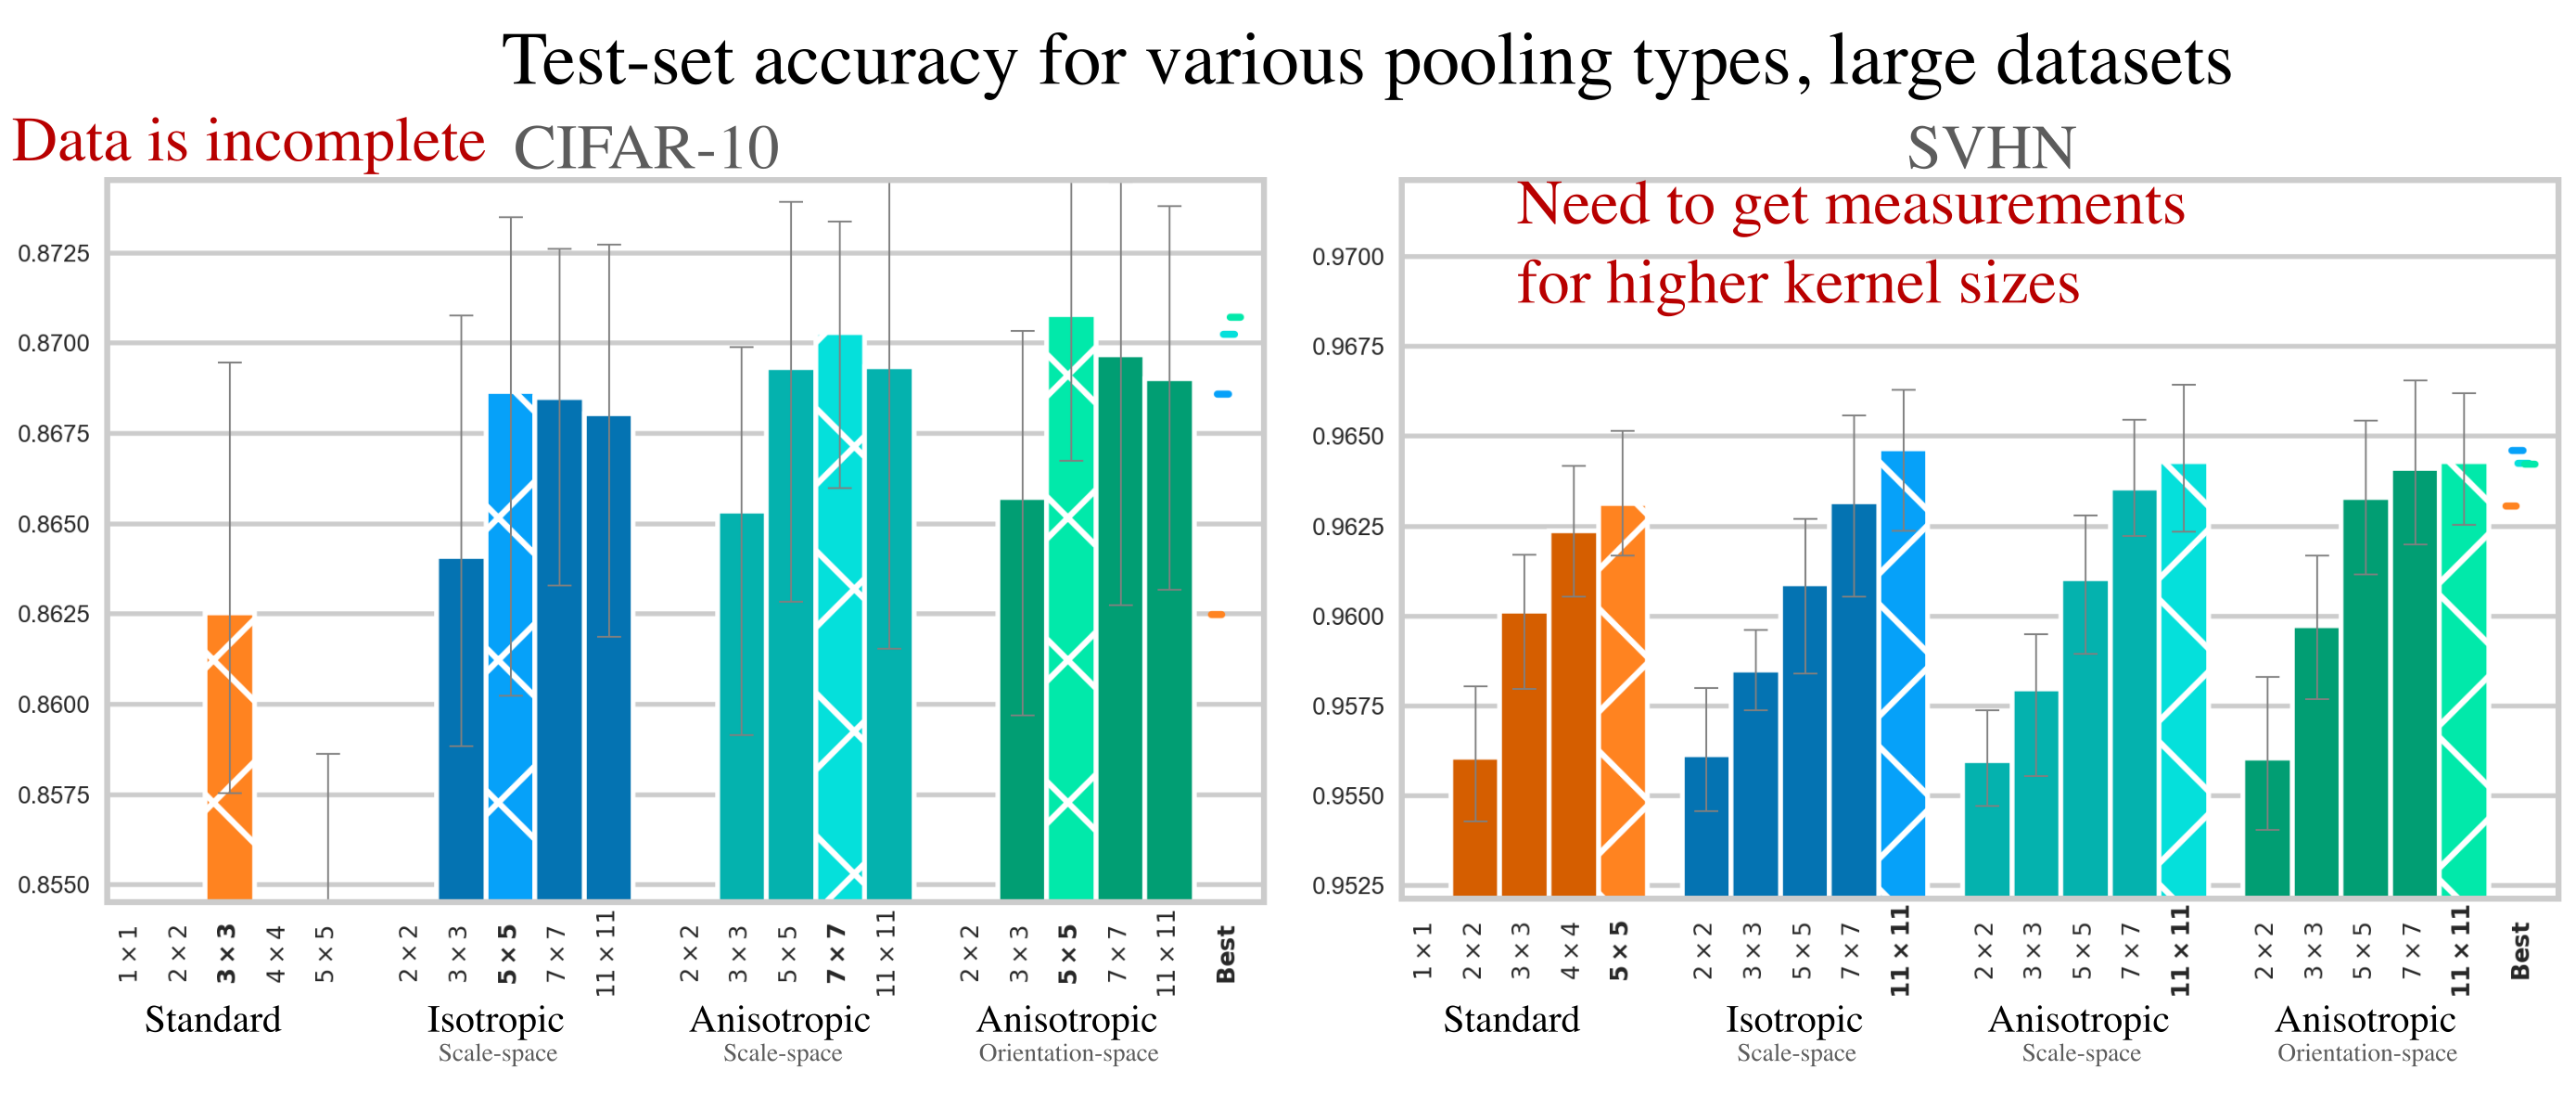
\includegraphics[width=1\textwidth]{figures/results-large.png}
  \caption{Accuracy (mean of 40) for model configurations on large datasets}
  \label{fig:res-large}
\end{figure}
\newpage
\begin{figure}[ht!]
	\center
  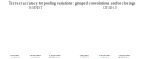
\includegraphics[width=1\textwidth]{figures/results-alt}
  \caption{Additional 'closing' and 'grouped' configurations (see Sec. \ref{sec:setup}), mean accuracy of 100 for K-MNIST and of 40 for CIFAR-10.}
  \label{fig:res-alt}
\end{figure}
\vspace{-0.4cm}
\section{Closings and grouped dilations}
Aside from the primary set of experiments, we can also examine the effects of using a closing $\boxclose$ instead of a dilation $\boxplus$, and/or using grouped convolutions (such that every pooling reduces over two channels). The results for K-MNIST and CIFAR-10 can be seen in Fig. \ref{fig:res-alt}, where the kernel sizes are selected based on previous results. We can see that using a closing significantly decreases performance (though closing remains slightly better than only subsampling),
while grouped convolutions also slightly decrease performance. Neither option appears to be a promising avenue for improvement, though more rigorous exploration of parameter combinations may show a different result.

\section{Training speed}
Though the execution speed and efficiency of the pooling layers is primarily discussed in the Extension report \cite{extension}, we can see in Fig. \ref{fig:res-timings} that the difference in training times (not including one-off compilation and model tracing times) between a standard max-pooling and a dilation is relatively minor. Depending on the use case, the additional increase in performance may, therefore, be worthwhile.
\comment{(These timings are outdated, and the final results will be faster)}
\begin{figure}[ht!]
	\center
  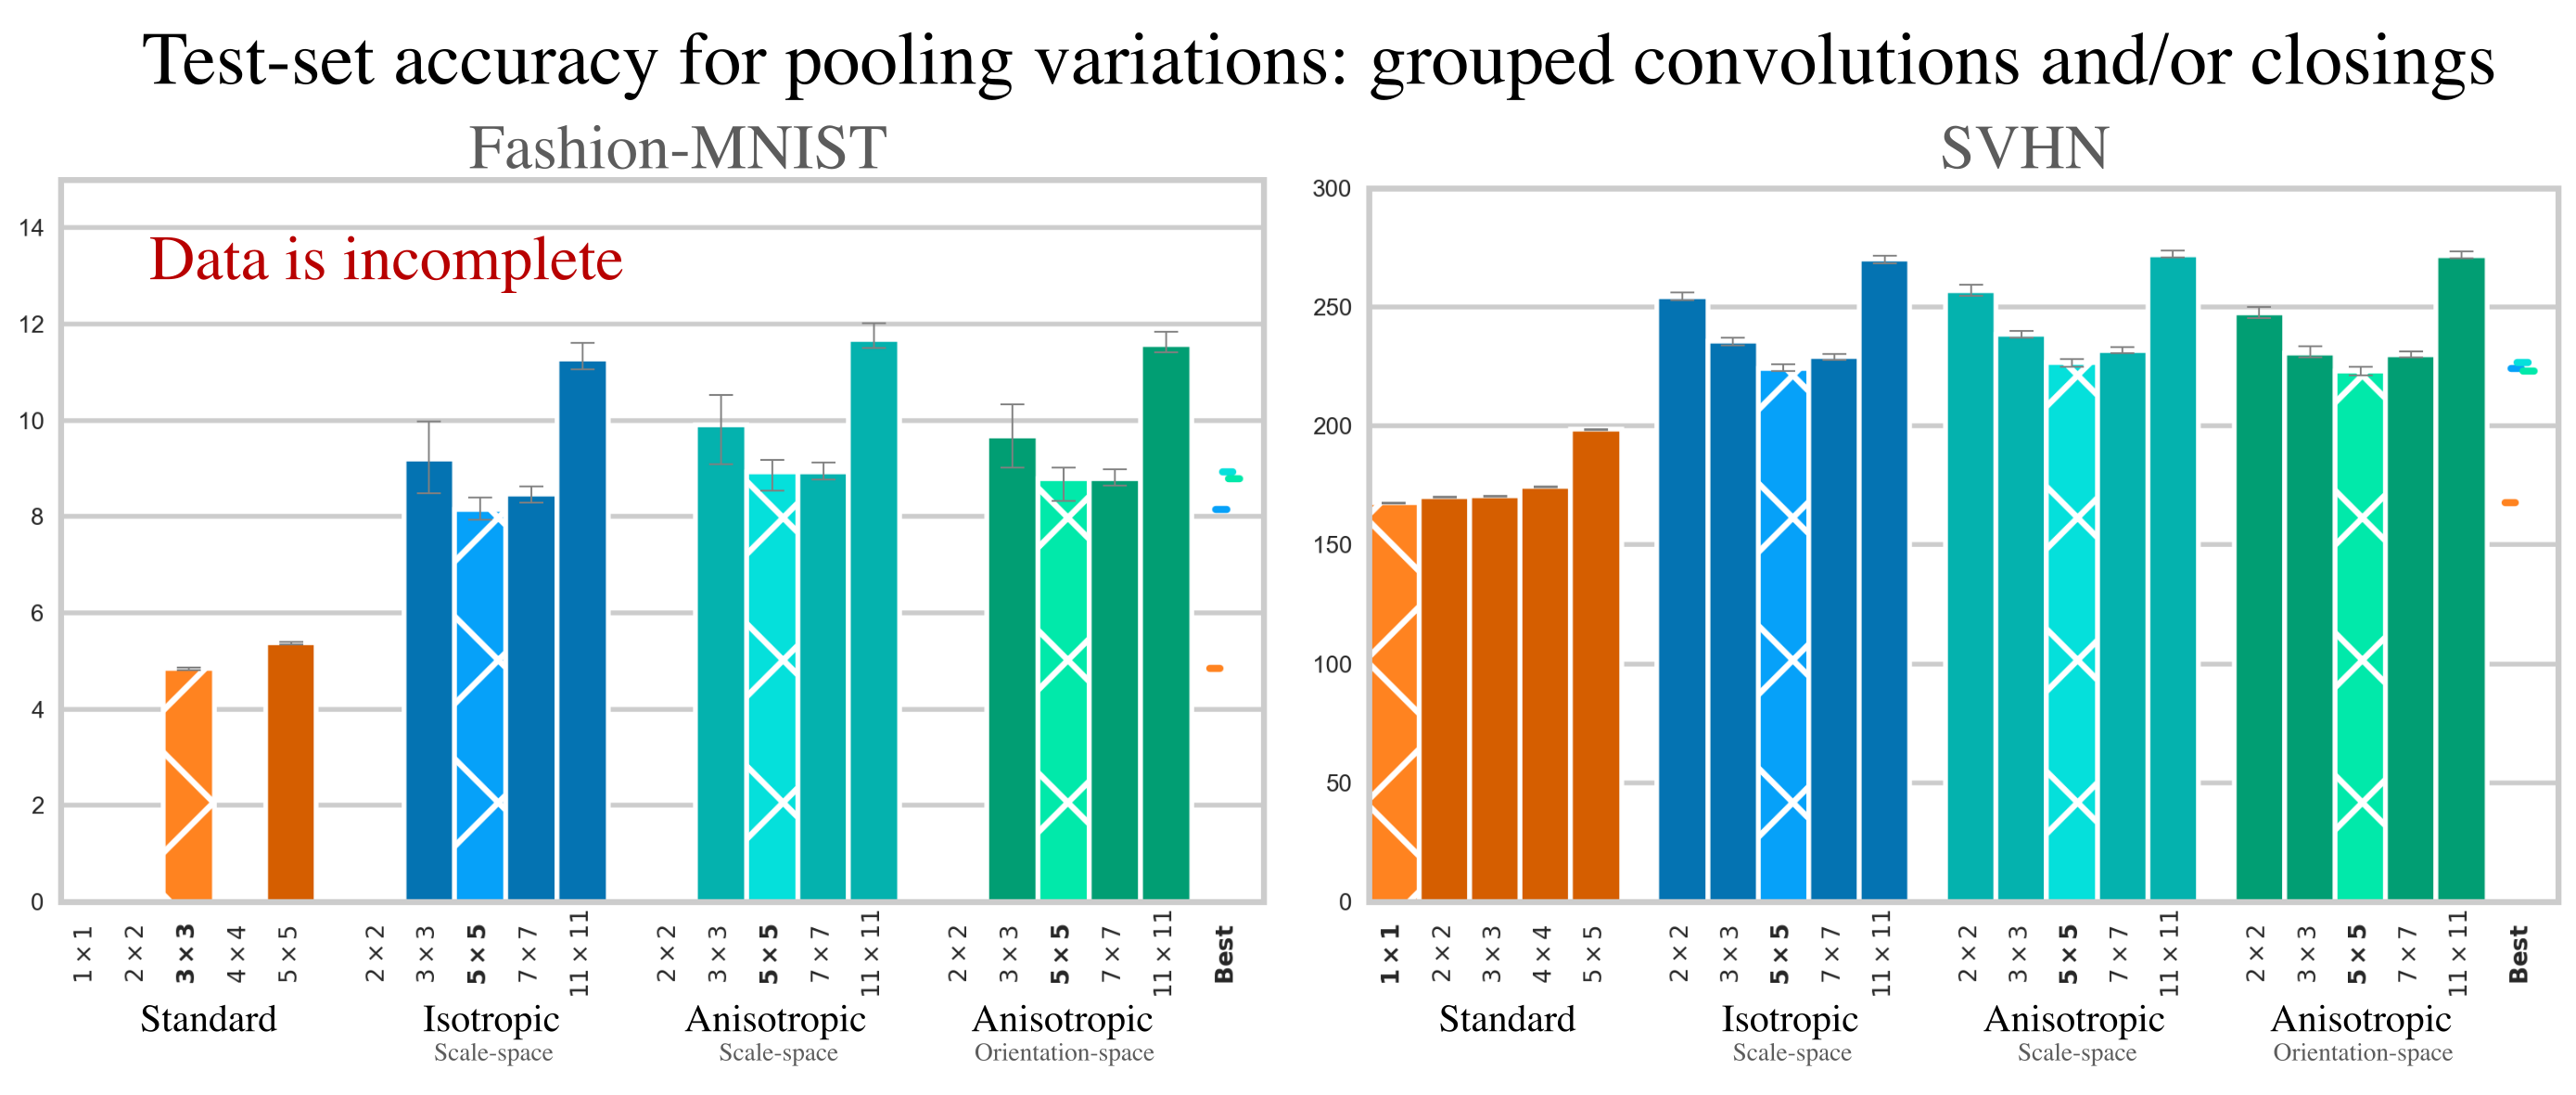
\includegraphics[width=1\textwidth]{figures/timings.png}
  \caption{Seconds per model trained for Fashion-MNIST and SVHN datasets}
  \label{fig:res-timings}
\end{figure}
\chapter{Conclusions}
\vspace{-1cm}
While it was previously shown that isotropic quadratic kernels can be used for dilations in the context of CNN max-pooling, this report has shown that:
\begin{itemize}
\setlength{\itemsep}{0pt}
	\item There are several methods for parameterising positive definite matrices for use in anisotropic quadratic kernels (see Sec. \ref{sec:learning-pdm}, Appendix \ref{sec:pearson}).
	\item Using such a method, anisotropic kernels can be learned via gradient descent (see Appendix \ref{sec:poc}) and applied for CNNs (see Sec. \ref{sec:setup}, Sec. \ref{sec:results}).
	\item For the datasets examined, anisotropic kernels showed performance similar to isotropic kernels and generally slightly better than standard max-poolings. Dilation-based models scored higher on 3 of the 4 datasets used but lower on Fashion-MNIST, while initialisation had limited impact.
	\item With careful implementation, training times of models using dilation can be kept close to models with standard max-poolings (see Extension \cite{extension}).
\end{itemize}
\vspace{-0.5cm}
\section{Discussion}
\label{sec:discussion}
CNNs are a powerful tool for machine learning with images; improvements can bring great value. While some sections of this report suggest positive outcomes when using dilations with anisotropic kernels, the results are not yet so conclusive as to be directly applicable in real-world scenarios.

The primary point of discussion for the results of this report would be the unexpectedly lacking performance of models using dilation-based pooling for Fashion-MNIST (see Fig. \ref{fig:res-small}). It is currently unknown what the cause of this would be, but possible explanations --- as mentioned --- include the LeNet-5 model being too small or Fashion-MNIST being unsuited for dilations.

Fashion-MNIST was also not included in the previous iterations of this research, where the datasets selected all showed positive results for dilation-based poolings. This suggests the existence of other datasets that may induce poor performance from dilation-based models and emphasises the importance of using varied datasets for evaluating a novel technique such as this.

Aside from using alternate datasets for gathering more insights into the behaviour of dilations, using structurally larger models and datasets (e.g.\ ImageNet) would also be important. Furthermore, many alternative parameterisations exist even within the space of models discussed in this report. It may be that using an alternative covariance parameterisation (e.g.\ Appendix \ref{sec:pearson}) may change the results, and it may be that alternative initialisation strategies could yield better outcomes (e.g.\ combining scale-space and orientation-space)

Due to the immense scope of possible model configurations, it may be that some important hyperparameters were missed. However, the steps taken in Sec. \ref{sec:setup} and \ref{sec:hyperparameters} have led to a baseline understanding of dilations for CNNs.



\newpage
\section{Further research}
Based on Sec. \ref{sec:discussion}, we identify the following directions for future research:
\begin{itemize}
\setlength{\itemsep}{1pt}
	\item What is the cause of the low performance for dilation-based models on Fashion-MNIST? Are there datasets that similarly induce poor results?
	\item Are the effects of dilation-based poolings also visible in large-scale CNNs?
	\item Do different methods for parameterising the covariance $\Sigma$ effect results? 
		  Are there other situations in which learnable covariances can be applied?
	\item How significant is the impact of variations in the initialisation of $\Sigma$? \\
	      Do mixes between orientation-space and scale-space initialisation (e.g.\ half of the kernels initialised by one, half by the other) have effects?
	 \item Outside of the domain of image classification, how well do dilation-based poolings perform? Can such poolings be applied to e.g.\ 3D data?
\end{itemize}
Additionally, while Appendix \ref{sec:nonlinconv} briefly touches on the topic, the possibilities of non-linear semifields for convolutional layers are also not fully explored.
Possible initial research directions adjacent to the topic might include:
\begin{itemize}
\setlength{\itemsep}{1pt}
	\item Which semifields are good candidates when replacing linear convolutions?
	\item Which parameters for such semifields yield usable results? Are there any that match or outperform a linear convolution?
	\item Are there specific types of datasets or tasks well-suited for non-linear convolutions?
\end{itemize}
\section{Contributions}
To briefly summarise the original contributions of this research, we have:
\begin{itemize}
\setlength{\itemsep}{0pt}
	\item Provided a coherent and visually aided overview of the relevant theory.
	\item Described two learnable parameterisations for covariance matrices $\Sigma$.
	\item Implemented efficient and replicable versions of the models described.
	\item Executed a clear performance analysis of anisotropic kernels for CNNs.
	\item Implemented highly efficient semifield convolutions (Extension \cite{extension}).
\end{itemize}

\section{Reproducibility}
All code to reproduce the results is available in a \href{https://github.com/p-adema/quadratic-conv}{\color{cyan}GitHub repository}; rerunning all experiments took approximately \comment{50?}\ hours on an NVIDIA RTX 5090.

Code for generating the graphs is also available, including the SVG files for all illustrations in the report and a copy of the report's \LaTeX \  code.
\section{Ethics}
While there are many ethical challenges involved in ensuring automated solutions for computer vision are not abused, this report is primarily theoretical and does not constitute a massive leap forward in state-of-the-art technology. As such, there is no reason to believe the models discussed could lead to new cases of abuse: any such cases were almost certainly possible beforehand.


\bibliographystyle{IEEEtran}
{\footnotesize \emergencystretch 1.5em \bibliography{references}}


\newpage
\chapter{Appendix}
\section{Redundancy of mirroring in $QDQ^T$}
\label{sec:red-mirr}
Suppose we had some symmetric $\Sigma \in \mathbb{R}^{2\times 2}$; we could then use orthogonal diagonalisation to write $\Sigma = QDQ^T$ for some orthogonal Q and diagonal D.

In \ref{sec:learning-pdm}, the claim was made that requiring $Q$ to be a rotation (and not a reflection) did not decrease the expressivity of the representation. In other words, all symmetric positive definite $\Sigma$ are representable as $RDR^T$ with R being a rotation. To show this, we can suppose some reflection $Q_\phi\in \mathbb{R}^{2\times 2}$, and see that $Q_\phi$ can be written as a rotation with angle $\phi$ (matrix $R_\phi$) of a reflection in the x-axis (from \cite{poole2015linear}):
\begin{align}
	Q_\phi=\begin{bmatrix}
		\cos \phi  &  \sin \phi  \\
		\sin \phi  &  -\cos \phi
	\end{bmatrix} &= \begin{bmatrix}
		\cos \phi  &  -\sin \phi  \\
		\sin \phi  &  \cos \phi
	\end{bmatrix} \begin{bmatrix}
		1  &  0  \\
		0  &  -1
	\end{bmatrix} = R_\phi \begin{bmatrix}
		1  &  0  \\
		0  &  -1
	\end{bmatrix} \label{eq:refl-rot}
\end{align}
Using \ref{eq:refl-rot}, we can see that the diagonal decomposition $\Sigma = QDQ^T$ with a $Q_\phi$ that represents a reflection can be rewritten to instead use a rotation $R_\phi$:
\begin{align}
	\Sigma&=Q_\phi DQ_\phi ^T \\
	&= \left(R_\phi \begin{bmatrix}
		1  &  0  \\
		0  &  -1
	\end{bmatrix}\right)D\left(R_\phi \begin{bmatrix}
		1  &  0  \\
		0  &  -1
	\end{bmatrix}\right)^T \\
	&= R_\phi \begin{bmatrix}
		1  &  0  \\
		0  &  -1
	\end{bmatrix} \begin{bmatrix}
		\sigma_1^2  &  0  \\
		0  &  \sigma_2^2
	\end{bmatrix} \begin{bmatrix}
		1  &  0  \\
		0  &  -1
	\end{bmatrix} R_\phi^T \\
%	&= R_\phi \begin{bmatrix}
%		\sigma_1^2  &  0  \\
%		0  &  -\sigma_2^2
%	\end{bmatrix} \begin{bmatrix}
%		1  &  0  \\
%		0  &  -1
%	\end{bmatrix} R_\phi^T \\
	&= R_\phi \begin{bmatrix}
		\sigma_1^2  &  0  \\
		0  &  -(-\sigma_2^2)
	\end{bmatrix} R_\phi^T \\
	&= R_\phi \begin{bmatrix}
		\sigma_1^2  &  0  \\
		0  &  \sigma_2^2
	\end{bmatrix} R_\phi^T \\
	&= R_\phi D R_\phi^T \\&&\qed\nonumber
\end{align}


\newpage
\section{Alternative parameterisation for $\Sigma \in \mathbb{R}^{2\times 2}$}
\label{sec:pearson}
A different way of parameterising a $2\times 2$ covariance matrix  would be to use the Pearson correlation coefficient $\rho$ instead of the angle $\phi$. 
We can then keep the covariance matrix in its Cholesky decomposed form, using a lower triangular $L$ such that $\Sigma=LL^T$. Then, for any $\boldsymbol{\theta}\in\mathbb{R}^3$, we can find the corresponding $L$:
\begin{align}
\textrm{Let }\boldsymbol{\theta}&=\begin{bmatrix}
	\theta_1\\
	\theta_2\\
	\theta_3\\
\end{bmatrix}=\begin{bmatrix}
	\log|\sigma_1| \\
	\log|\sigma_2|\\
	\tan\rho\\
\end{bmatrix}, \textrm{ then a valid $\Sigma$ would be} \\
	\Sigma &= \begin{bmatrix}
 \sigma_1^2 & \sigma_1\sigma_2\rho \\
  \sigma_1\sigma_2\rho & \sigma_2^2 \\
\end{bmatrix}
= LL^T = \begin{bmatrix}
 l_{11} & 0 \\
  l_{21} & l_{22} \\
\end{bmatrix}\begin{bmatrix}
 l_{11} & l_{21} \\
  0 & l_{22} \\
\end{bmatrix}\\
&=\begin{bmatrix}
 l_{11}^2 & l_{11}l_{21} \\
  l_{11}l_{21} & l_{21}^2 + l_{22}^2 \\
\end{bmatrix}\hspace{0.5cm}\\
\textrm{As such,}&\textrm{ we know that:}\nonumber\\
	l_{11} &= \sqrt{\sigma_1^2} =\sigma_1=\exp(\theta_1)\\
	l_{21} &= \frac{\sigma_1\sigma_2\rho}{\sigma_1}=\sigma_2\rho=\exp(\theta_2)\tanh(\theta_3) \\
%	l_{21}^2 + l_{22}^2 &= \sigma_2^2 \textrm{, so}\\
	l_{22} &= \sqrt{\sigma_2^2 - \sigma_2\rho} = \sqrt{\exp(2\theta_2)-\exp(\theta_2)\tanh(\theta_3)}
\end{align}
which is then a valid parameterisation for the Cholesky decomposed form for a $2\times 2$ positive definite matrix\footnote{To extend this parameterisation for higher dimensions, see the  Cholesky-Banachiewicz algorithm for the Cholesky decomposition}. If we keep the covariance matrix in this triangular form, we can see that the quadratic form can be calculated in an efficient manner:

(based on the PyTorch code for the multivariate normal PDF)
\begin{align}
	\mathbf{x}^T\Sigma^{-1}\mathbf{x}
	&= \mathbf{x}^T(LL^T)^{-1}\mathbf{x}\\
	&= \mathbf{x}^T(L^T)^{-1}L^{-1}\mathbf{x}\\
	&= \mathbf{x}^T(L^{-1})^{T}L^{-1}\mathbf{x}\\
	&= ((L^{-1})\mathbf{x})^T(L^{-1}\mathbf{x})\\
	&= (L^{-1}\mathbf{x})\cdot(L^{-1}\mathbf{x})\\
\textrm{Suppose }\mathbf{b}&=L^{-1}\mathbf{x}, \textrm{ then} \nonumber\\
	L\mathbf{b}&=\mathbf{x}, \textrm{ so}\nonumber\\
	\mathbf{b}&= \textsc{solve-triangular}(L, \mathbf{x})\\
	\mathbf{x}^T\Sigma^{-1}\mathbf{x} &= \mathbf{b}\cdot\mathbf{b}
\end{align}
where $\textsc{solve-triangular}$ performs efficient backsubstitution to avoid computing the inverse. This method is significantly (>5x) faster on the CPU it was tested on while still showing modest performance improvements on the GPU\footnote{In eager mode, i.e.\ without \lstinline{torch.compile} or CUDA-graphs enabled. When using CUDA-graphs, the performance difference is negligible (as allocation overhead disappears).} it was tested on ($\sim 10\%$). However, interpretation of the Pearson correlation coefficient may be more challenging compared to interpreting the angular offset of the first primary axis, and when properly compiled/captured using CUDA-graphs the performance difference vanishes, so it was chosen to instead parameterise $\Sigma$ with the angle $\phi$.

\newpage
\section{Hyperparameter tuning }
\label{sec:hyperparameters}
To determine an appropriate learning rate and epoch count for training the models, a validation split was made for each dataset from the training data. 70\% of the training data was marked for training models for the tuning process, while the remaining 30\% would be used to select the best learning rate and epoch count.
In Fig. \ref{fig:tuning}, we can see the results, showing that a learning rate around 0.003 or 0.004 is typically best, with the number of epochs required for training varying greatly based on the complexity of the dataset and task. 

For convenience, Table \ref{table:hyperparameters} is repeated here and shows the selected values:

\begin{table}[!htbp]
\centering
\begin{tabular}{l|*4c}
\toprule
Hyperparameter & K-MNIST & Fashion-MNIST & CIFAR-10 & SVHN\\
\midrule
Batch size & \multicolumn{4}{c}{1024 (saturates GPU compute)}\\
Optimiser   &  \multicolumn{4}{c}{Adam, default parameters except \textsc{lr}} \\
Learning rate & 0.004 & 0.003 & 0.004 & 0.003 \\
Epochs & 30 & 80 & 150 & 250 \\
\bottomrule
\end{tabular}
\caption{Hyperparameters used when training models on datasets (copy).}
\end{table}

\begin{figure}[h!]
	\center
  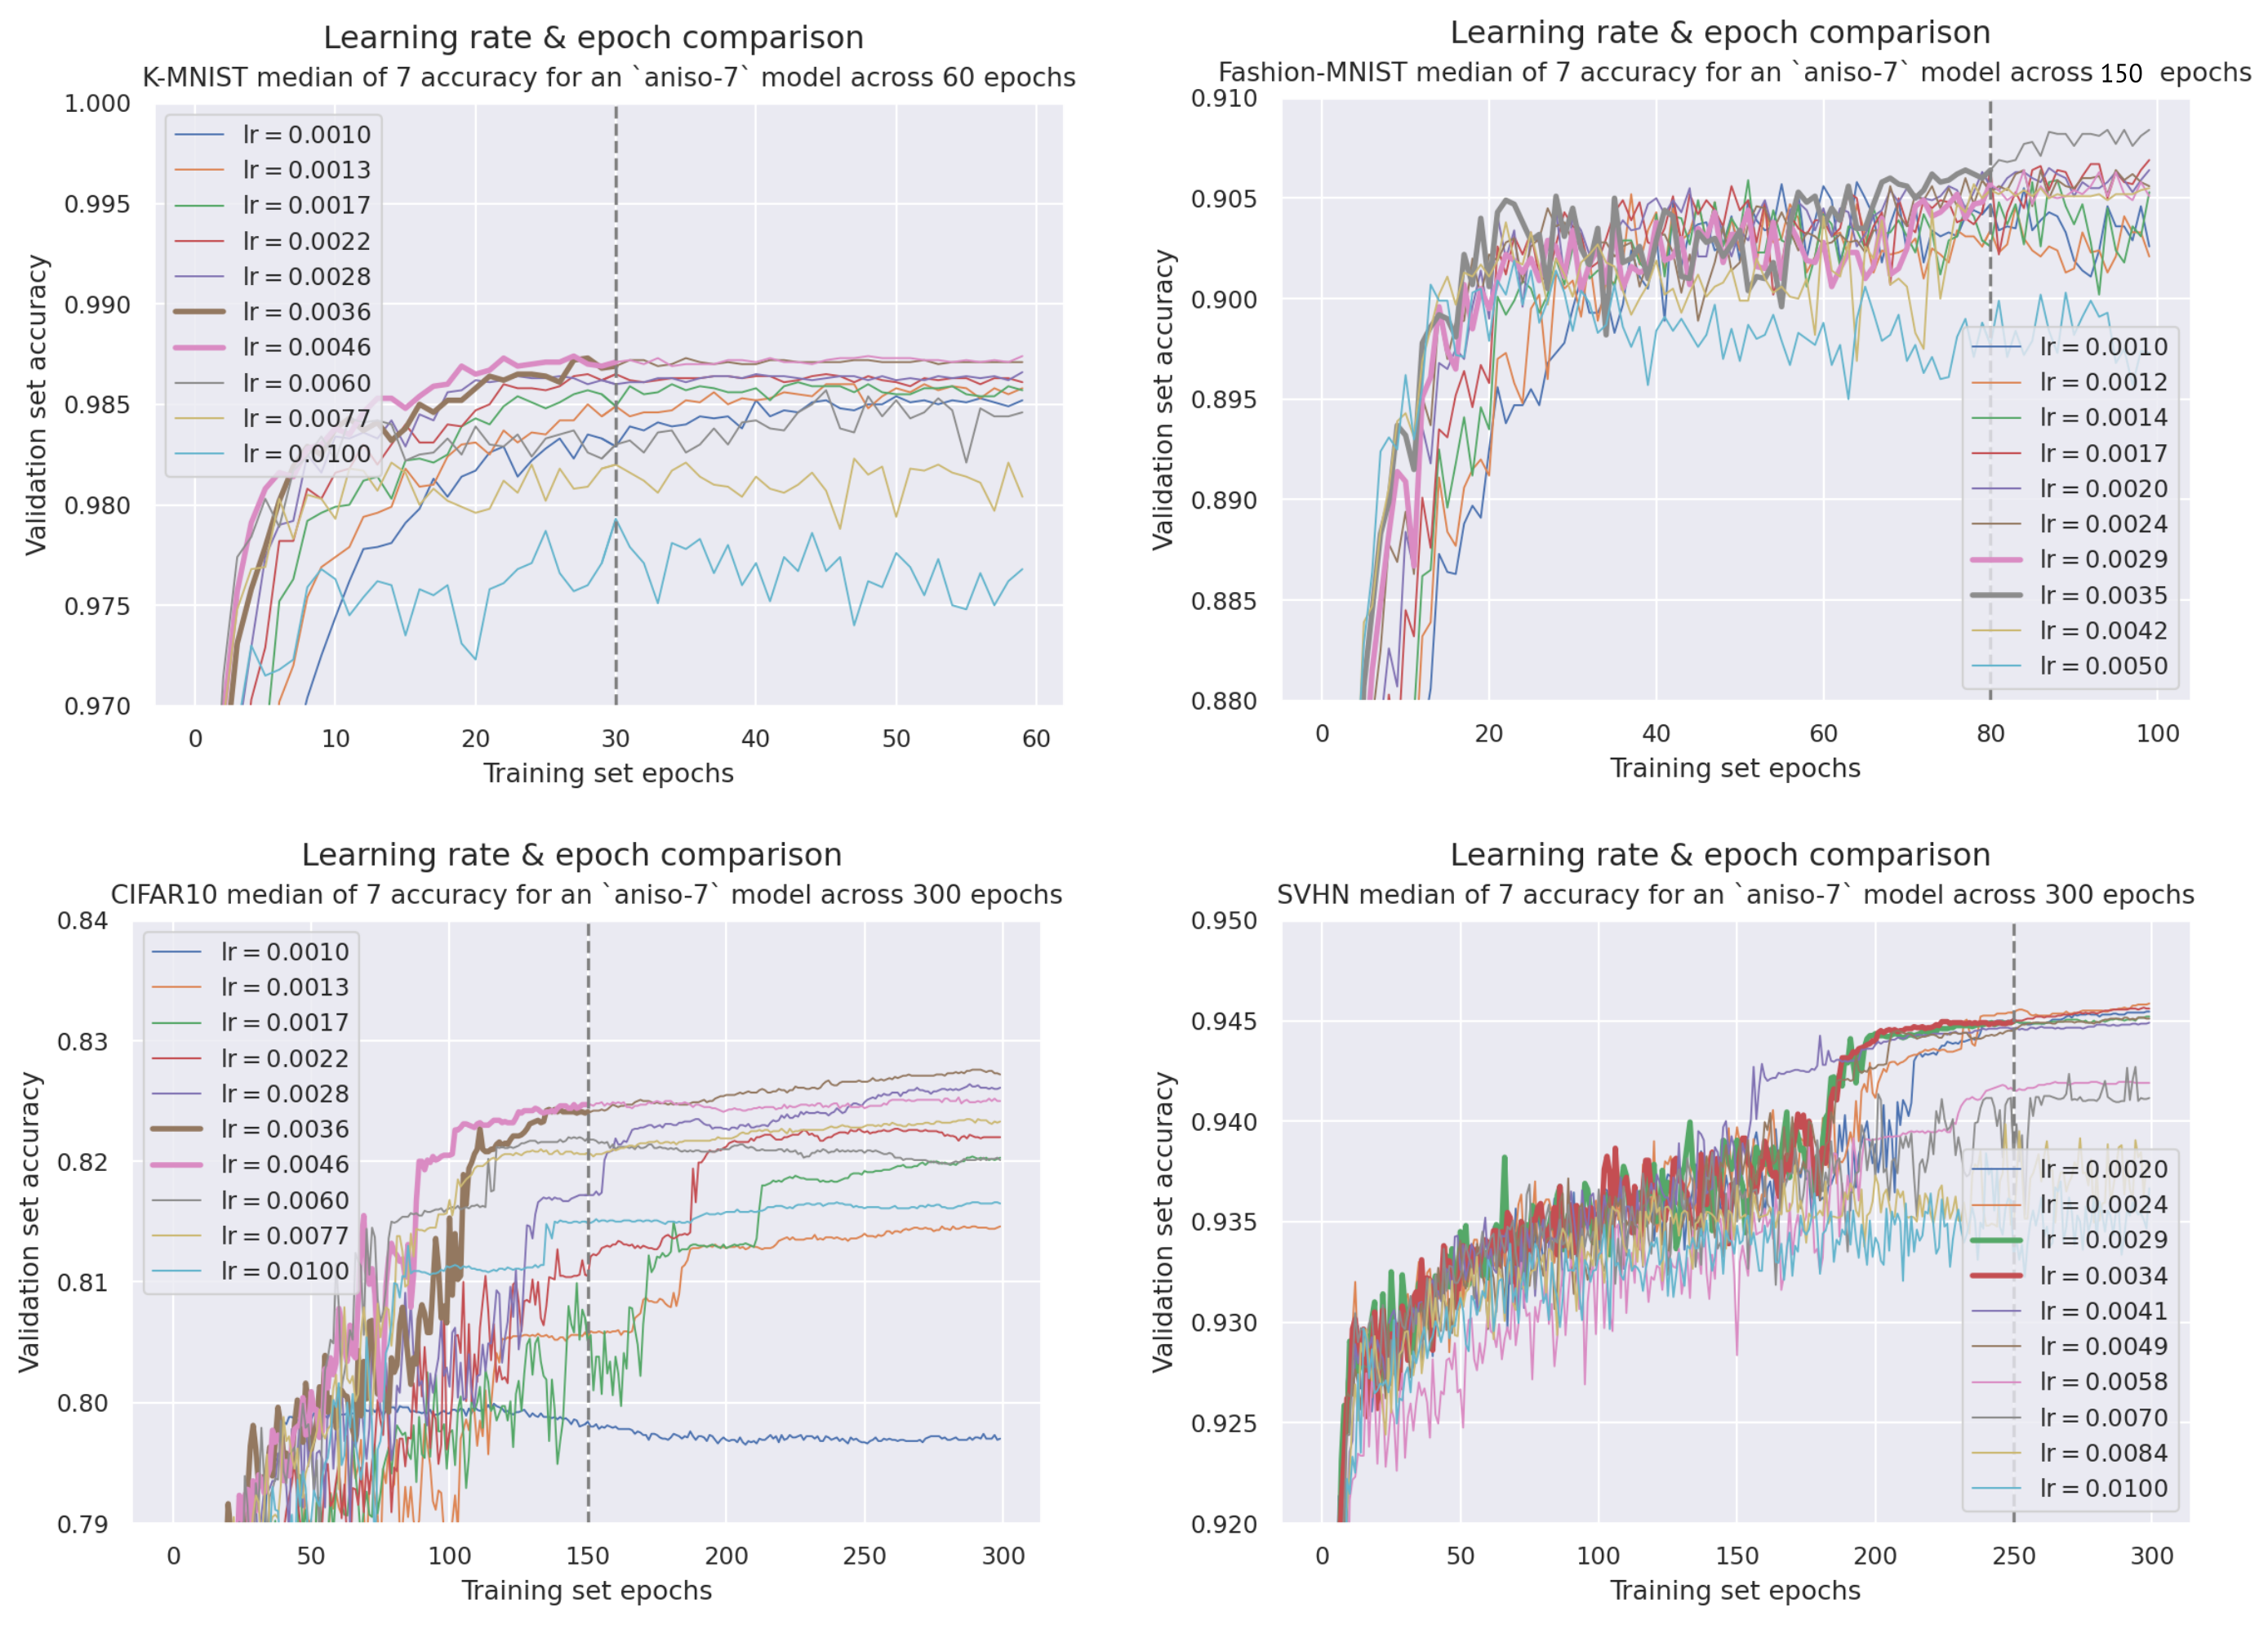
\includegraphics[width=\textwidth]{figures/learning_rates.png}
  \caption{Hyperparameter tuning results, with selected learning rates as bold lines and the epoch cutoff marked with a dashed grey line.}
  \label{fig:tuning}
\end{figure}

\noindent
More complex hyperparameter tuning, such as adjusting the type of optimiser or the other (e.g.\ momentum) parameters of the optimiser, was considered. However, additional tuning did not seem necessary to achieve a result sufficiently representative of optimally tuned performance. It is expected that further adjustments would yield higher accuracies but that these gains would be felt approximately equally amongst all pooling types (it would likely not change the conclusions of the report).


\newpage
\section{Experiments with $R_p$ and $L_{\mu+}$ convolutions }
\label{sec:nonlinconv}
As a brief foray into the use of alternate semifields for standard (linear) convolutional layers, a simple experiment using the K-MNIST dataset was conducted. Here, two variations on two highly-scoring models were attempted. The two base models were both LeNet-5 models, with the first having a $3\times3$ standard max-pooling, while the second had a $7\times7$ anisotropic (orientation space) pooling. The two variations were to replace the linear convolution layers in the LeNet model with either $\textcircled{$*$}_{R_p}$ or $\textcircled{$*$}_{L_\mu}$, while also varying the parameter $p$ / $\mu$ (see Sec. \ref{sec:non-morph}).
The results can be seen in Fig. \ref{fig:nonlinconv}, where neither variation seemed to be able to fit to the data (save for $R_1$, which is the same as the linear field). These initial results suggest that alternatives to the linear field are likely numerically unstable: it is possible that an alternative configuration would yield positive results, but the experiments, as shown, are negative on the usage of alternatives to the linear field for convolutional layers in a CNN.

\begin{figure}[h!]
	\center
  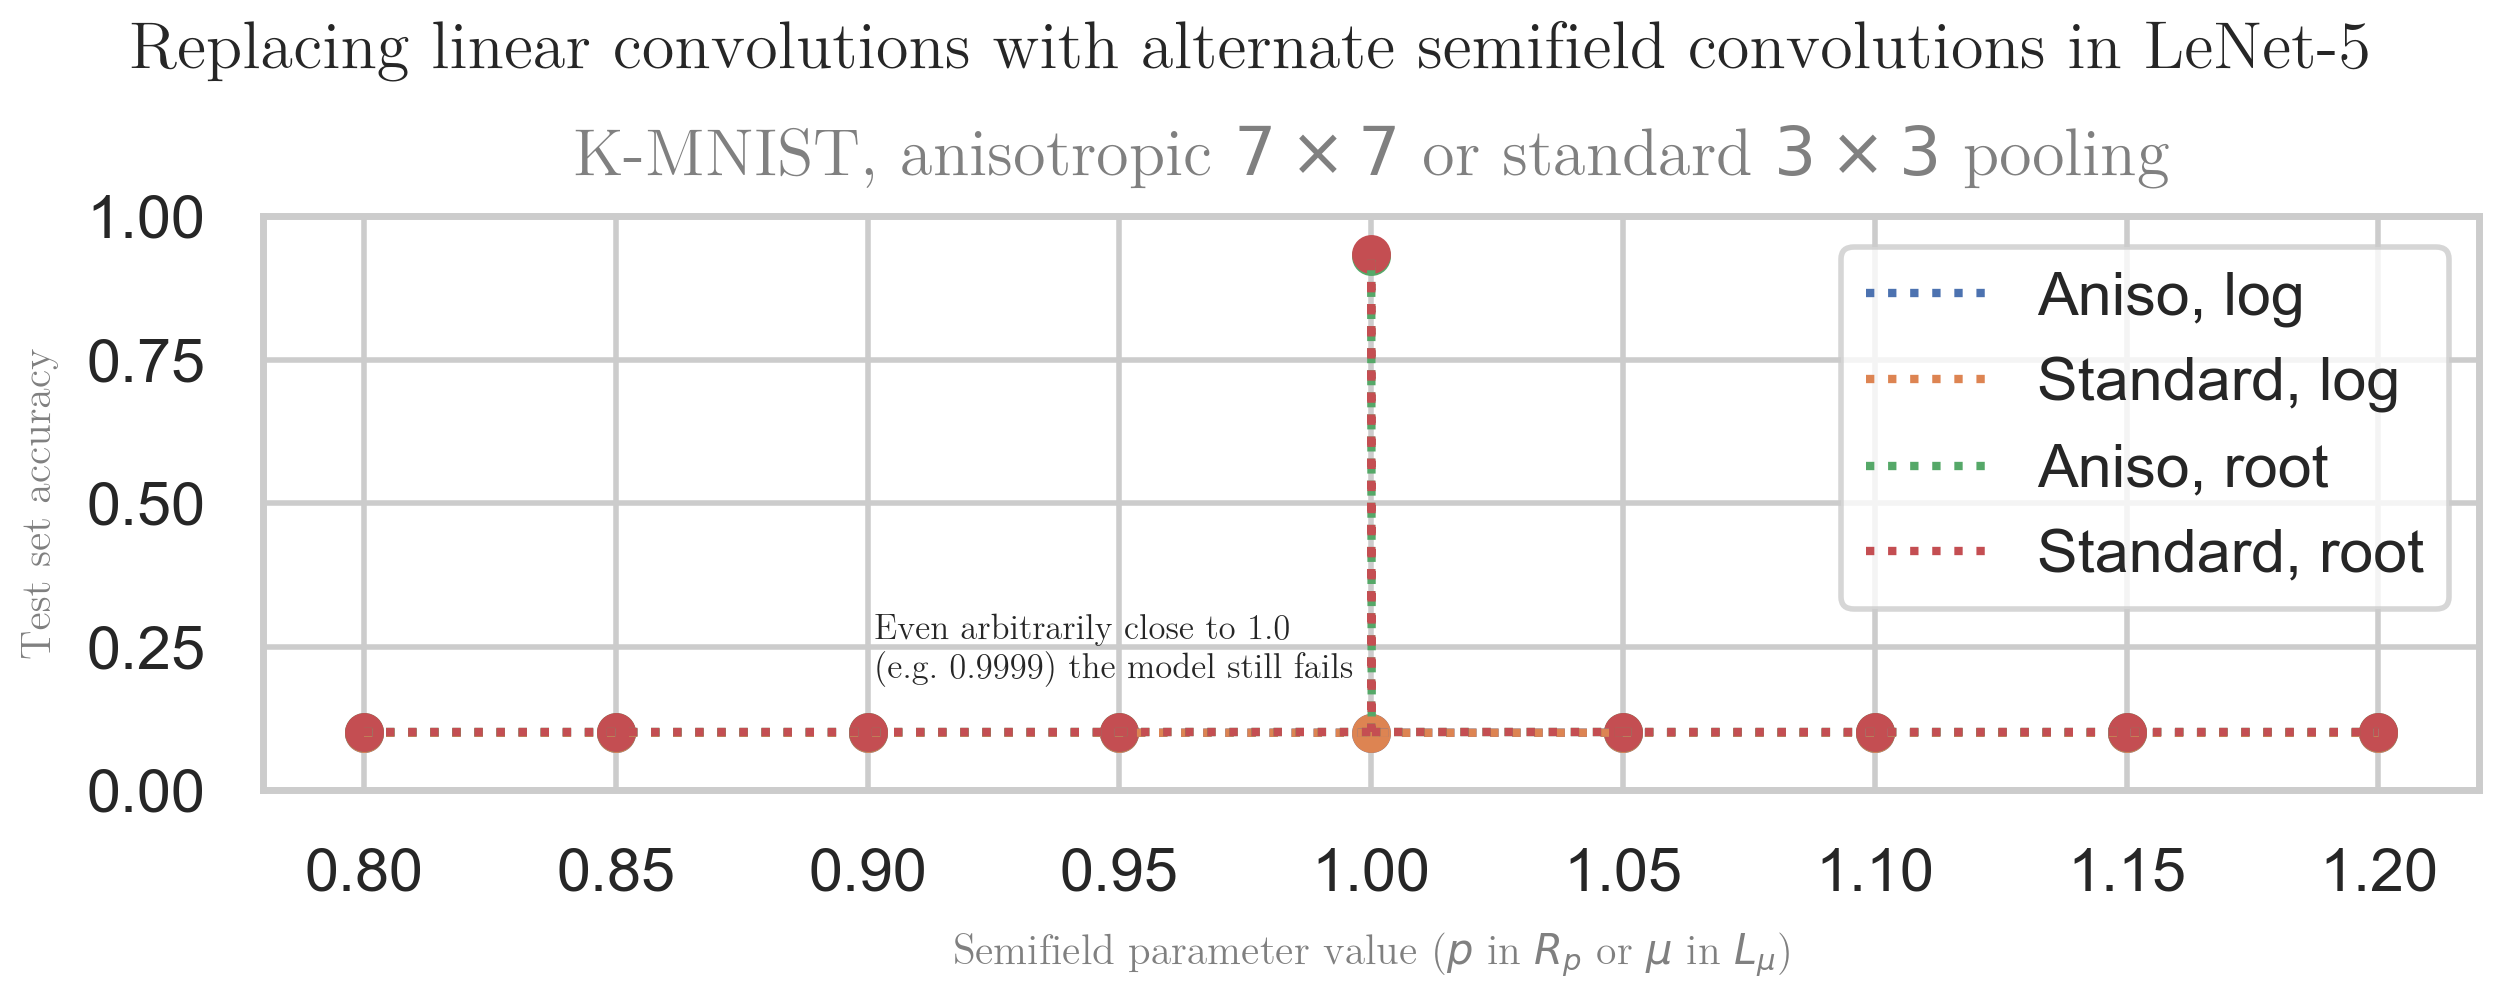
\includegraphics[width=\textwidth]{figures/results_nonlin.png}
  \caption{Results of nonlinear convolutions $R_p$ and $L_\mu$ for various $p$ and $\mu$ around 1. The pooling type does not seem to have a large effect (lines overlap).}
  \label{fig:nonlinconv}
\end{figure}
\vspace{-0.8cm}
\section{Learnability Proof of Concept}
\label{sec:poc}
Similar to Section 3.1 of \cite{thierrybsc}, this section aims to verify that the kernels and convolutions used in the experiments can converge to a target value via gradient descent. While \cite{thierrybsc} chose to visualise the outputs of the dilation changing, this is impractical for 2D data. Instead, we choose to visualise the kernel itself. Aside from the output format, the method will remain the same; given a target kernel and some random input data, the result of a dilation with the target kernel is compared to the result with a learnable kernel. The resulting loss is backpropagated, and after sufficient steps of gradient descent, the learnable kernel will approximate the target kernel: see Fig. \ref{fig:poc}.


\begin{figure}[h!]
	\center
  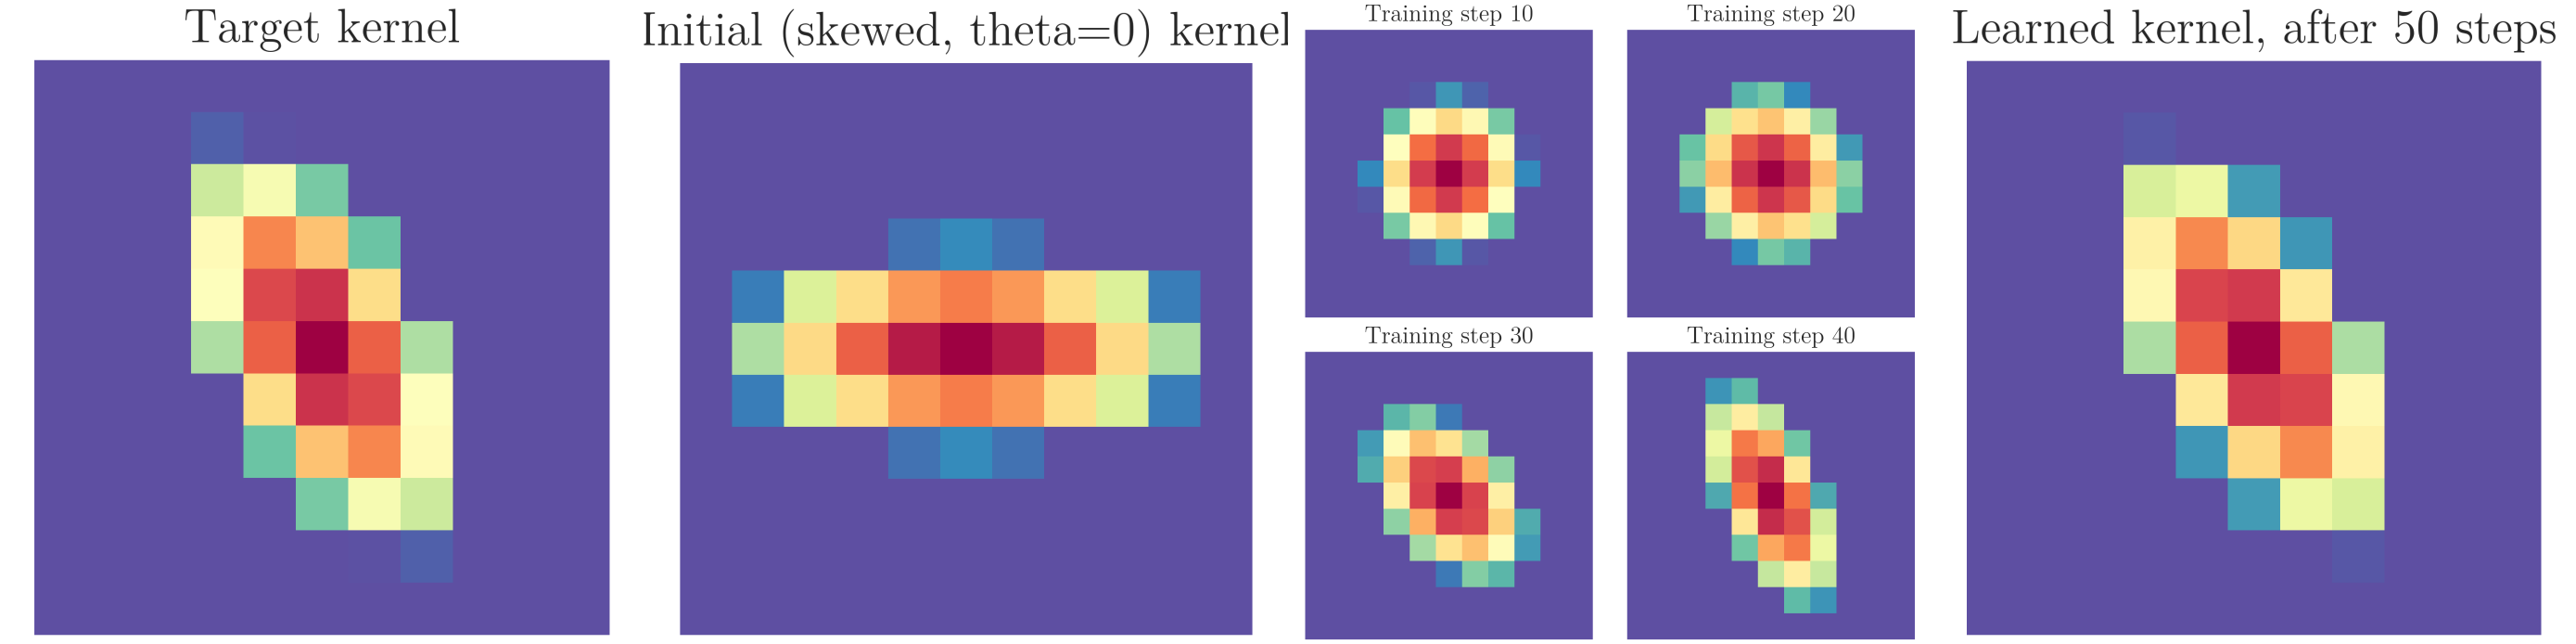
\includegraphics[width=\textwidth]{figures/poc.png}
  \caption{Anisotropic kernels can be learned via gradient descent.}
  \label{fig:poc}
\end{figure}
\end{document}
